\documentclass[1p]{elsarticle_modified}
%\bibliographystyle{elsarticle-num}

%\usepackage[colorlinks]{hyperref}
%\usepackage{abbrmath_seonhwa} %\Abb, \Ascr, \Acal ,\Abf, \Afrak
\usepackage{amsfonts}
\usepackage{amssymb}
\usepackage{amsmath}
\usepackage{amsthm}
\usepackage{scalefnt}
\usepackage{amsbsy}
\usepackage{kotex}
\usepackage{caption}
\usepackage{subfig}
\usepackage{color}
\usepackage{graphicx}
\usepackage{xcolor} %% white, black, red, green, blue, cyan, magenta, yellow
\usepackage{float}
\usepackage{setspace}
\usepackage{hyperref}

\usepackage{tikz}
\usetikzlibrary{arrows}

\usepackage{multirow}
\usepackage{array} % fixed length table
\usepackage{hhline}

%%%%%%%%%%%%%%%%%%%%%
\makeatletter
\renewcommand*\env@matrix[1][\arraystretch]{%
	\edef\arraystretch{#1}%
	\hskip -\arraycolsep
	\let\@ifnextchar\new@ifnextchar
	\array{*\c@MaxMatrixCols c}}
\makeatother %https://tex.stackexchange.com/questions/14071/how-can-i-increase-the-line-spacing-in-a-matrix
%%%%%%%%%%%%%%%

\usepackage[normalem]{ulem}

\newcommand{\msout}[1]{\ifmmode\text{\sout{\ensuremath{#1}}}\else\sout{#1}\fi}
%SOURCE: \msout is \stkout macro in https://tex.stackexchange.com/questions/20609/strikeout-in-math-mode

\newcommand{\cancel}[1]{
	\ifmmode
	{\color{red}\msout{#1}}
	\else
	{\color{red}\sout{#1}}
	\fi
}

\newcommand{\add}[1]{
	{\color{blue}\uwave{#1}}
}

\newcommand{\replace}[2]{
	\ifmmode
	{\color{red}\msout{#1}}{\color{blue}\uwave{#2}}
	\else
	{\color{red}\sout{#1}}{\color{blue}\uwave{#2}}
	\fi
}

\newcommand{\Sol}{\mathcal{S}} %segment
\newcommand{\D}{D} %diagram
\newcommand{\A}{\mathcal{A}} %arc


%%%%%%%%%%%%%%%%%%%%%%%%%%%%%5 test

\def\sl{\operatorname{\textup{SL}}(2,\Cbb)}
\def\psl{\operatorname{\textup{PSL}}(2,\Cbb)}
\def\quan{\mkern 1mu \triangleright \mkern 1mu}

\theoremstyle{definition}
\newtheorem{thm}{Theorem}[section]
\newtheorem{prop}[thm]{Proposition}
\newtheorem{lem}[thm]{Lemma}
\newtheorem{ques}[thm]{Question}
\newtheorem{cor}[thm]{Corollary}
\newtheorem{defn}[thm]{Definition}
\newtheorem{exam}[thm]{Example}
\newtheorem{rmk}[thm]{Remark}
\newtheorem{alg}[thm]{Algorithm}

\newcommand{\I}{\sqrt{-1}}
\begin{document}

%\begin{frontmatter}
%
%\title{Boundary parabolic representations of knots up to 8 crossings}
%
%%% Group authors per affiliation:
%\author{Yunhi Cho} 
%\address{Department of Mathematics, University of Seoul, Seoul, Korea}
%\ead{yhcho@uos.ac.kr}
%
%
%\author{Seonhwa Kim} %\fnref{s_kim}}
%\address{Center for Geometry and Physics, Institute for Basic Science, Pohang, 37673, Korea}
%\ead{ryeona17@ibs.re.kr}
%
%\author{Hyuk Kim}
%\address{Department of Mathematical Sciences, Seoul National University, Seoul 08826, Korea}
%\ead{hyukkim@snu.ac.kr}
%
%\author{Seokbeom Yoon}
%\address{Department of Mathematical Sciences, Seoul National University, Seoul, 08826,  Korea}
%\ead{sbyoon15@snu.ac.kr}
%
%\begin{abstract}
%We find all boundary parabolic representation of knots up to 8 crossings.
%
%\end{abstract}
%\begin{keyword}
%    \MSC[2010] 57M25 
%\end{keyword}
%
%\end{frontmatter}

%\linenumbers
%\tableofcontents
%
\newcommand\colored[1]{\textcolor{white}{\rule[-0.35ex]{0.8em}{1.4ex}}\kern-0.8em\color{red} #1}%
%\newcommand\colored[1]{\textcolor{white}{ #1}\kern-2.17ex	\textcolor{white}{ #1}\kern-1.81ex	\textcolor{white}{ #1}\kern-2.15ex\color{red}#1	}

{\Large $\underline{12a_{0393}~(K12a_{0393})}$}

\setlength{\tabcolsep}{10pt}
\renewcommand{\arraystretch}{1.6}
\vspace{1cm}\begin{tabular}{m{100pt}>{\centering\arraybackslash}m{274pt}}
\multirow{5}{120pt}{
	\centering
	\includegraphics[width=112pt]{../../../GIT/diagram.site/Diagrams/png/1194_12a_0393.png}\\
\ \ \ A knot diagram\footnotemark}&
\allowdisplaybreaks
\textbf{Linearized knot diagam} \\
\cline{2-2}
 &
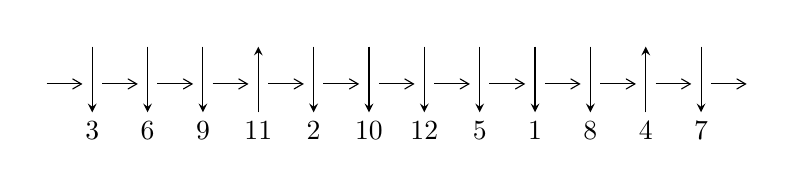
\begin{tikzpicture}[x=20pt, y=17pt]
	% nodes
	\node (C0) at (0, 0) {};
	\node (C1) at (1, 0) {};
	\node (C1U) at (1, +1) {};
	\node (C1D) at (1, -1) {3};

	\node (C2) at (2, 0) {};
	\node (C2U) at (2, +1) {};
	\node (C2D) at (2, -1) {6};

	\node (C3) at (3, 0) {};
	\node (C3U) at (3, +1) {};
	\node (C3D) at (3, -1) {9};

	\node (C4) at (4, 0) {};
	\node (C4U) at (4, +1) {};
	\node (C4D) at (4, -1) {11};

	\node (C5) at (5, 0) {};
	\node (C5U) at (5, +1) {};
	\node (C5D) at (5, -1) {2};

	\node (C6) at (6, 0) {};
	\node (C6U) at (6, +1) {};
	\node (C6D) at (6, -1) {10};

	\node (C7) at (7, 0) {};
	\node (C7U) at (7, +1) {};
	\node (C7D) at (7, -1) {12};

	\node (C8) at (8, 0) {};
	\node (C8U) at (8, +1) {};
	\node (C8D) at (8, -1) {5};

	\node (C9) at (9, 0) {};
	\node (C9U) at (9, +1) {};
	\node (C9D) at (9, -1) {1};

	\node (C10) at (10, 0) {};
	\node (C10U) at (10, +1) {};
	\node (C10D) at (10, -1) {8};

	\node (C11) at (11, 0) {};
	\node (C11U) at (11, +1) {};
	\node (C11D) at (11, -1) {4};

	\node (C12) at (12, 0) {};
	\node (C12U) at (12, +1) {};
	\node (C12D) at (12, -1) {7};
	\node (C13) at (13, 0) {};

	% arrows
	\draw[->,>={angle 60}]
	(C0) edge (C1) (C1) edge (C2) (C2) edge (C3) (C3) edge (C4) (C4) edge (C5) (C5) edge (C6) (C6) edge (C7) (C7) edge (C8) (C8) edge (C9) (C9) edge (C10) (C10) edge (C11) (C11) edge (C12) (C12) edge (C13) ;	\draw[->,>=stealth]
	(C1U) edge (C1D) (C2U) edge (C2D) (C3U) edge (C3D) (C4D) edge (C4U) (C5U) edge (C5D) (C6U) edge (C6D) (C7U) edge (C7D) (C8U) edge (C8D) (C9U) edge (C9D) (C10U) edge (C10D) (C11D) edge (C11U) (C12U) edge (C12D) ;
	\end{tikzpicture} \\
\hhline{~~} \\& 
\textbf{Solving Sequence} \\ \cline{2-2} 
 &
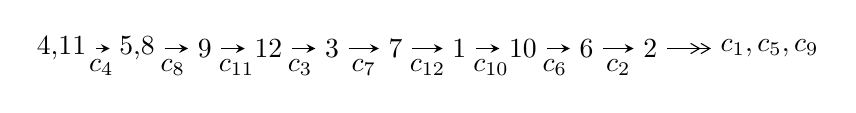
\begin{tikzpicture}[x=23pt, y=7pt]
	% node
	\node (A0) at (-1/8, 0) {4,11};
	\node (A1) at (17/16, 0) {5,8};
	\node (A2) at (17/8, 0) {9};
	\node (A3) at (25/8, 0) {12};
	\node (A4) at (33/8, 0) {3};
	\node (A5) at (41/8, 0) {7};
	\node (A6) at (49/8, 0) {1};
	\node (A7) at (57/8, 0) {10};
	\node (A8) at (65/8, 0) {6};
	\node (A9) at (73/8, 0) {2};
	\node (C1) at (1/2, -1) {$c_{4}$};
	\node (C2) at (13/8, -1) {$c_{8}$};
	\node (C3) at (21/8, -1) {$c_{11}$};
	\node (C4) at (29/8, -1) {$c_{3}$};
	\node (C5) at (37/8, -1) {$c_{7}$};
	\node (C6) at (45/8, -1) {$c_{12}$};
	\node (C7) at (53/8, -1) {$c_{10}$};
	\node (C8) at (61/8, -1) {$c_{6}$};
	\node (C9) at (69/8, -1) {$c_{2}$};
	\node (A10) at (11, 0) {$c_{1},c_{5},c_{9}$};

	% edge
	\draw[->,>=stealth]	
	(A0) edge (A1) (A1) edge (A2) (A2) edge (A3) (A3) edge (A4) (A4) edge (A5) (A5) edge (A6) (A6) edge (A7) (A7) edge (A8) (A8) edge (A9) ;
	\draw[->>,>={angle 60}]	
	(A9) edge (A10);
\end{tikzpicture} \\ 

\end{tabular} \\

\footnotetext{
The image of knot diagram is generated by the software ``\textbf{Draw programme}" developed by Andrew Bartholomew(\url{http://www.layer8.co.uk/maths/draw/index.htm\#Running-draw}), where we modified some parts for our purpose(\url{https://github.com/CATsTAILs/LinksPainter}).
}\phantom \\ \newline 
\centering \textbf{Ideals for irreducible components\footnotemark of $X_{\text{par}}$} 
 
\begin{align*}
I^u_{1}&=\langle 
2.16436\times10^{820} u^{170}-7.16961\times10^{820} u^{169}+\cdots+1.69091\times10^{821} b-3.15772\times10^{824},\\
\phantom{I^u_{1}}&\phantom{= \langle  }2.26218\times10^{824} u^{170}-1.11946\times10^{825} u^{169}+\cdots+1.66706\times10^{825} a-9.23150\times10^{828},\\
\phantom{I^u_{1}}&\phantom{= \langle  }u^{171}-2 u^{170}+\cdots+4671 u+9859\rangle \\
I^u_{2}&=\langle 
-1.47468\times10^{22} u^{40}-9.65322\times10^{22} u^{39}+\cdots+1.45371\times10^{21} b-2.19717\times10^{23},\\
\phantom{I^u_{2}}&\phantom{= \langle  }4.08057\times10^{20} u^{40}-2.19309\times10^{23} u^{39}+\cdots+1.45371\times10^{21} a-5.58423\times10^{23},\;u^{41}+u^{40}+\cdots+16 u^2+1\rangle \\
\\
\end{align*}
\raggedright * 2 irreducible components of $\dim_{\mathbb{C}}=0$, with total 212 representations.\\
\footnotetext{All coefficients of polynomials are rational numbers. But the coefficients are sometimes approximated in decimal forms when there is not enough margin.}
\newpage
\renewcommand{\arraystretch}{1}
\centering \section*{I. $I^u_{1}= \langle 2.16\times10^{820} u^{170}-7.17\times10^{820} u^{169}+\cdots+1.69\times10^{821} b-3.16\times10^{824},\;2.26\times10^{824} u^{170}-1.12\times10^{825} u^{169}+\cdots+1.67\times10^{825} a-9.23\times10^{828},\;u^{171}-2 u^{170}+\cdots+4671 u+9859 \rangle$}
\flushleft \textbf{(i) Arc colorings}\\
\begin{tabular}{m{7pt} m{180pt} m{7pt} m{180pt} }
\flushright $a_{4}=$&$\begin{pmatrix}1\\0\end{pmatrix}$ \\
\flushright $a_{11}=$&$\begin{pmatrix}0\\u\end{pmatrix}$ \\
\flushright $a_{5}=$&$\begin{pmatrix}1\\- u^2\end{pmatrix}$ \\
\flushright $a_{8}=$&$\begin{pmatrix}-0.135698 u^{170}+0.671518 u^{169}+\cdots+3689.38 u+5537.58\\-0.128000 u^{170}+0.424010 u^{169}+\cdots+603.968 u+1867.47\end{pmatrix}$ \\
\flushright $a_{9}=$&$\begin{pmatrix}-0.319349 u^{170}+1.10997 u^{169}+\cdots+3616.53 u+7614.90\\-0.305108 u^{170}+0.760621 u^{169}+\cdots-874.296 u+2568.95\end{pmatrix}$ \\
\flushright $a_{12}=$&$\begin{pmatrix}u\\u\end{pmatrix}$ \\
\flushright $a_{3}=$&$\begin{pmatrix}-0.632479 u^{170}+1.87166 u^{169}+\cdots+2965.36 u+12068.5\\-0.678695 u^{170}+1.60465 u^{169}+\cdots-1882.78 u+7820.21\end{pmatrix}$ \\
\flushright $a_{7}=$&$\begin{pmatrix}-0.231129 u^{170}+0.997129 u^{169}+\cdots+4697.68 u+7825.97\\-0.223431 u^{170}+0.749621 u^{169}+\cdots+1612.26 u+4155.86\end{pmatrix}$ \\
\flushright $a_{1}=$&$\begin{pmatrix}0.697139 u^{170}-1.39628 u^{169}+\cdots+5773.34 u-2258.59\\0.597639 u^{170}-1.19850 u^{169}+\cdots+4279.61 u-2387.93\end{pmatrix}$ \\
\flushright $a_{10}=$&$\begin{pmatrix}-1.50364 u^{170}+2.34391 u^{169}+\cdots-21755.3 u-2660.63\\-0.880774 u^{170}+1.08735 u^{169}+\cdots-16968.6 u-4931.27\end{pmatrix}$ \\
\flushright $a_{6}=$&$\begin{pmatrix}-0.828240 u^{170}+0.786031 u^{169}+\cdots-18991.7 u-7508.20\\-0.511994 u^{170}+0.263356 u^{169}+\cdots-14937.7 u-7521.50\end{pmatrix}$ \\
\flushright $a_{2}=$&$\begin{pmatrix}-0.482941 u^{170}+0.744544 u^{169}+\cdots-5025.31 u+1650.19\\-0.152795 u^{170}+0.157950 u^{169}+\cdots-2168.84 u+595.438\end{pmatrix}$\\&\end{tabular}
\flushleft \textbf{(ii) Obstruction class $= -1$}\\~\\
\flushleft \textbf{(iii) Cusp Shapes $= 1.62396 u^{170}-2.54230 u^{169}+\cdots+19935.1 u+2386.95$}\\~\\
\newpage\renewcommand{\arraystretch}{1}
\flushleft \textbf{(iv) u-Polynomials at the component}\newline \\
\begin{tabular}{m{50pt}|m{274pt}}
Crossings & \hspace{64pt}u-Polynomials at each crossing \\
\hline $$\begin{aligned}c_{1}\end{aligned}$$&$\begin{aligned}
&u^{171}+78 u^{170}+\cdots+2521 u+49
\end{aligned}$\\
\hline $$\begin{aligned}c_{2},c_{5}\end{aligned}$$&$\begin{aligned}
&u^{171}+4 u^{170}+\cdots+111 u+7
\end{aligned}$\\
\hline $$\begin{aligned}c_{3}\end{aligned}$$&$\begin{aligned}
&u^{171}- u^{170}+\cdots-404430848 u+29671424
\end{aligned}$\\
\hline $$\begin{aligned}c_{4},c_{11}\end{aligned}$$&$\begin{aligned}
&u^{171}-2 u^{170}+\cdots+4671 u+9859
\end{aligned}$\\
\hline $$\begin{aligned}c_{6}\end{aligned}$$&$\begin{aligned}
&u^{171}-3 u^{170}+\cdots+37835 u+2123
\end{aligned}$\\
\hline $$\begin{aligned}c_{7},c_{12}\end{aligned}$$&$\begin{aligned}
&u^{171}+2 u^{170}+\cdots-528354 u+43591
\end{aligned}$\\
\hline $$\begin{aligned}c_{8}\end{aligned}$$&$\begin{aligned}
&u^{171}+5 u^{170}+\cdots+61115146 u+5504449
\end{aligned}$\\
\hline $$\begin{aligned}c_{9}\end{aligned}$$&$\begin{aligned}
&u^{171}+8 u^{170}+\cdots-25208926 u+28448137
\end{aligned}$\\
\hline $$\begin{aligned}c_{10}\end{aligned}$$&$\begin{aligned}
&u^{171}+8 u^{170}+\cdots+208397 u+48167
\end{aligned}$\\
\hline
\end{tabular}\\~\\
\newpage\renewcommand{\arraystretch}{1}
\flushleft \textbf{(v) Riley Polynomials at the component}\newline \\
\begin{tabular}{m{50pt}|m{274pt}}
Crossings & \hspace{64pt}Riley Polynomials at each crossing \\
\hline $$\begin{aligned}c_{1}\end{aligned}$$&$\begin{aligned}
&y^{171}+46 y^{170}+\cdots+1499345 y-2401
\end{aligned}$\\
\hline $$\begin{aligned}c_{2},c_{5}\end{aligned}$$&$\begin{aligned}
&y^{171}-78 y^{170}+\cdots+2521 y-49
\end{aligned}$\\
\hline $$\begin{aligned}c_{3}\end{aligned}$$&$\begin{aligned}
&y^{171}+15 y^{170}+\cdots-5219403641651200 y-880393402187776
\end{aligned}$\\
\hline $$\begin{aligned}c_{4},c_{11}\end{aligned}$$&$\begin{aligned}
&y^{171}+92 y^{170}+\cdots-778002993 y-97199881
\end{aligned}$\\
\hline $$\begin{aligned}c_{6}\end{aligned}$$&$\begin{aligned}
&y^{171}+41 y^{170}+\cdots+1410817697 y-4507129
\end{aligned}$\\
\hline $$\begin{aligned}c_{7},c_{12}\end{aligned}$$&$\begin{aligned}
&y^{171}+126 y^{170}+\cdots-157098337588 y-1900175281
\end{aligned}$\\
\hline $$\begin{aligned}c_{8}\end{aligned}$$&$\begin{aligned}
&y^{171}-47 y^{170}+\cdots+638582748630030 y-30298958793601
\end{aligned}$\\
\hline $$\begin{aligned}c_{9}\end{aligned}$$&$\begin{aligned}
&y^{171}+46 y^{170}+\cdots-25343801026808550 y-809296498770769
\end{aligned}$\\
\hline $$\begin{aligned}c_{10}\end{aligned}$$&$\begin{aligned}
&y^{171}-10 y^{170}+\cdots+163308109881 y-2320059889
\end{aligned}$\\
\hline
\end{tabular}\\~\\
\newpage\flushleft \textbf{(vi) Complex Volumes and Cusp Shapes}
$$\begin{array}{c|c|c}  
\text{Solutions to }I^u_{1}& \I (\text{vol} + \sqrt{-1}CS) & \text{Cusp shape}\\
 \hline 
\begin{aligned}
u &= \phantom{-}0.522816 + 0.862319 I \\
a &= -1.38476 + 0.76073 I \\
b &= -0.23131 + 1.56919 I\end{aligned}
 & \phantom{-}2.60729 - 1.52346 I & \phantom{-0.000000 } 0 \\ \hline\begin{aligned}
u &= \phantom{-}0.522816 - 0.862319 I \\
a &= -1.38476 - 0.76073 I \\
b &= -0.23131 - 1.56919 I\end{aligned}
 & \phantom{-}2.60729 + 1.52346 I & \phantom{-0.000000 } 0 \\ \hline\begin{aligned}
u &= \phantom{-}0.909426 + 0.435762 I \\
a &= -0.119413 - 0.866013 I \\
b &= \phantom{-}0.390430 + 0.327958 I\end{aligned}
 & \phantom{-}4.06706 + 0.85033 I & \phantom{-0.000000 } 0 \\ \hline\begin{aligned}
u &= \phantom{-}0.909426 - 0.435762 I \\
a &= -0.119413 + 0.866013 I \\
b &= \phantom{-}0.390430 - 0.327958 I\end{aligned}
 & \phantom{-}4.06706 - 0.85033 I & \phantom{-0.000000 } 0 \\ \hline\begin{aligned}
u &= -0.408687 + 0.900797 I \\
a &= \phantom{-}0.513684 - 0.597894 I \\
b &= \phantom{-}1.42692 - 1.76208 I\end{aligned}
 & \phantom{-}5.28982 - 5.58495 I & \phantom{-0.000000 } 0 \\ \hline\begin{aligned}
u &= -0.408687 - 0.900797 I \\
a &= \phantom{-}0.513684 + 0.597894 I \\
b &= \phantom{-}1.42692 + 1.76208 I\end{aligned}
 & \phantom{-}5.28982 + 5.58495 I & \phantom{-0.000000 } 0 \\ \hline\begin{aligned}
u &= \phantom{-}0.360268 + 0.917654 I \\
a &= \phantom{-}0.520539 + 1.062350 I \\
b &= \phantom{-}1.47874 + 1.40925 I\end{aligned}
 & -0.0998941 - 0.0172681 I & \phantom{-0.000000 } 0 \\ \hline\begin{aligned}
u &= \phantom{-}0.360268 - 0.917654 I \\
a &= \phantom{-}0.520539 - 1.062350 I \\
b &= \phantom{-}1.47874 - 1.40925 I\end{aligned}
 & -0.0998941 + 0.0172681 I & \phantom{-0.000000 } 0 \\ \hline\begin{aligned}
u &= \phantom{-}0.245163 + 0.991099 I \\
a &= -0.008836 - 0.982029 I \\
b &= -1.27704 - 1.77108 I\end{aligned}
 & -1.25424 + 5.11311 I & \phantom{-0.000000 } 0 \\ \hline\begin{aligned}
u &= \phantom{-}0.245163 - 0.991099 I \\
a &= -0.008836 + 0.982029 I \\
b &= -1.27704 + 1.77108 I\end{aligned}
 & -1.25424 - 5.11311 I & \phantom{-0.000000 } 0\\
 \hline 
 \end{array}$$\newpage$$\begin{array}{c|c|c}  
\text{Solutions to }I^u_{1}& \I (\text{vol} + \sqrt{-1}CS) & \text{Cusp shape}\\
 \hline 
\begin{aligned}
u &= -0.959438 + 0.132908 I \\
a &= \phantom{-}0.752972 + 0.258045 I \\
b &= -0.185217 + 0.308499 I\end{aligned}
 & -3.70458 - 0.52517 I & \phantom{-0.000000 } 0 \\ \hline\begin{aligned}
u &= -0.959438 - 0.132908 I \\
a &= \phantom{-}0.752972 - 0.258045 I \\
b &= -0.185217 - 0.308499 I\end{aligned}
 & -3.70458 + 0.52517 I & \phantom{-0.000000 } 0 \\ \hline\begin{aligned}
u &= \phantom{-}0.450784 + 0.931709 I \\
a &= -0.641768 - 0.682341 I \\
b &= -1.45912 - 1.78519 I\end{aligned}
 & \phantom{-}3.89033 + 11.06030 I & \phantom{-0.000000 } 0 \\ \hline\begin{aligned}
u &= \phantom{-}0.450784 - 0.931709 I \\
a &= -0.641768 + 0.682341 I \\
b &= -1.45912 + 1.78519 I\end{aligned}
 & \phantom{-}3.89033 - 11.06030 I & \phantom{-0.000000 } 0 \\ \hline\begin{aligned}
u &= \phantom{-}0.143513 + 0.952277 I \\
a &= -0.126743 + 0.262061 I \\
b &= \phantom{-}0.268539 + 0.771000 I\end{aligned}
 & -0.77746 + 1.36820 I & \phantom{-0.000000 } 0 \\ \hline\begin{aligned}
u &= \phantom{-}0.143513 - 0.952277 I \\
a &= -0.126743 - 0.262061 I \\
b &= \phantom{-}0.268539 - 0.771000 I\end{aligned}
 & -0.77746 - 1.36820 I & \phantom{-0.000000 } 0 \\ \hline\begin{aligned}
u &= -0.327368 + 0.999695 I \\
a &= -0.525772 + 0.390138 I \\
b &= -0.047209 + 1.285440 I\end{aligned}
 & -0.24255 + 1.97395 I & \phantom{-0.000000 } 0 \\ \hline\begin{aligned}
u &= -0.327368 - 0.999695 I \\
a &= -0.525772 - 0.390138 I \\
b &= -0.047209 - 1.285440 I\end{aligned}
 & -0.24255 - 1.97395 I & \phantom{-0.000000 } 0 \\ \hline\begin{aligned}
u &= -0.892591 + 0.560383 I \\
a &= \phantom{-}0.126506 - 0.724879 I \\
b &= -0.481848 + 0.396131 I\end{aligned}
 & \phantom{-}3.64192 - 5.10552 I & \phantom{-0.000000 } 0 \\ \hline\begin{aligned}
u &= -0.892591 - 0.560383 I \\
a &= \phantom{-}0.126506 + 0.724879 I \\
b &= -0.481848 - 0.396131 I\end{aligned}
 & \phantom{-}3.64192 + 5.10552 I & \phantom{-0.000000 } 0\\
 \hline 
 \end{array}$$\newpage$$\begin{array}{c|c|c}  
\text{Solutions to }I^u_{1}& \I (\text{vol} + \sqrt{-1}CS) & \text{Cusp shape}\\
 \hline 
\begin{aligned}
u &= -0.372716 + 0.988870 I \\
a &= \phantom{-}0.460916 - 1.169530 I \\
b &= -0.23905 - 1.70014 I\end{aligned}
 & -2.77213 - 1.78404 I & \phantom{-0.000000 } 0 \\ \hline\begin{aligned}
u &= -0.372716 - 0.988870 I \\
a &= \phantom{-}0.460916 + 1.169530 I \\
b &= -0.23905 + 1.70014 I\end{aligned}
 & -2.77213 + 1.78404 I & \phantom{-0.000000 } 0 \\ \hline\begin{aligned}
u &= \phantom{-}0.274336 + 1.024780 I \\
a &= \phantom{-}0.571806 + 0.302014 I \\
b &= -1.38226 + 0.57658 I\end{aligned}
 & \phantom{-}0.50931 + 6.41538 I & \phantom{-0.000000 } 0 \\ \hline\begin{aligned}
u &= \phantom{-}0.274336 - 1.024780 I \\
a &= \phantom{-}0.571806 - 0.302014 I \\
b &= -1.38226 - 0.57658 I\end{aligned}
 & \phantom{-}0.50931 - 6.41538 I & \phantom{-0.000000 } 0 \\ \hline\begin{aligned}
u &= -0.254872 + 0.898952 I \\
a &= -0.959077 + 0.046936 I \\
b &= \phantom{-}1.022820 - 0.168338 I\end{aligned}
 & \phantom{-}3.63281 - 0.53934 I & \phantom{-0.000000 } 0 \\ \hline\begin{aligned}
u &= -0.254872 - 0.898952 I \\
a &= -0.959077 - 0.046936 I \\
b &= \phantom{-}1.022820 + 0.168338 I\end{aligned}
 & \phantom{-}3.63281 + 0.53934 I & \phantom{-0.000000 } 0 \\ \hline\begin{aligned}
u &= -0.766566 + 0.742347 I \\
a &= \phantom{-}0.187282 - 0.294692 I \\
b &= -0.574949 + 0.697972 I\end{aligned}
 & \phantom{-}3.14382 - 0.82943 I & \phantom{-0.000000 } 0 \\ \hline\begin{aligned}
u &= -0.766566 - 0.742347 I \\
a &= \phantom{-}0.187282 + 0.294692 I \\
b &= -0.574949 - 0.697972 I\end{aligned}
 & \phantom{-}3.14382 + 0.82943 I & \phantom{-0.000000 } 0 \\ \hline\begin{aligned}
u &= \phantom{-}0.665772 + 0.843021 I \\
a &= -0.209489 + 0.100833 I \\
b &= \phantom{-}0.612905 + 0.963363 I\end{aligned}
 & \phantom{-}2.99332 + 4.80623 I & \phantom{-0.000000 } 0 \\ \hline\begin{aligned}
u &= \phantom{-}0.665772 - 0.843021 I \\
a &= -0.209489 - 0.100833 I \\
b &= \phantom{-}0.612905 - 0.963363 I\end{aligned}
 & \phantom{-}2.99332 - 4.80623 I & \phantom{-0.000000 } 0\\
 \hline 
 \end{array}$$\newpage$$\begin{array}{c|c|c}  
\text{Solutions to }I^u_{1}& \I (\text{vol} + \sqrt{-1}CS) & \text{Cusp shape}\\
 \hline 
\begin{aligned}
u &= \phantom{-}0.292872 + 0.873573 I \\
a &= \phantom{-}0.78424 + 1.95800 I \\
b &= \phantom{-}1.87599 + 2.23240 I\end{aligned}
 & \phantom{-}2.88872 - 6.87672 I & \phantom{-0.000000 } 0 \\ \hline\begin{aligned}
u &= \phantom{-}0.292872 - 0.873573 I \\
a &= \phantom{-}0.78424 - 1.95800 I \\
b &= \phantom{-}1.87599 - 2.23240 I\end{aligned}
 & \phantom{-}2.88872 + 6.87672 I & \phantom{-0.000000 } 0 \\ \hline\begin{aligned}
u &= -0.422237 + 0.814113 I \\
a &= \phantom{-}1.75628 + 0.42376 I \\
b &= \phantom{-}0.505283 + 1.221520 I\end{aligned}
 & \phantom{-}4.82984 - 2.83468 I & \phantom{-0.000000 } 0 \\ \hline\begin{aligned}
u &= -0.422237 - 0.814113 I \\
a &= \phantom{-}1.75628 - 0.42376 I \\
b &= \phantom{-}0.505283 - 1.221520 I\end{aligned}
 & \phantom{-}4.82984 + 2.83468 I & \phantom{-0.000000 } 0 \\ \hline\begin{aligned}
u &= -0.314631 + 0.855483 I \\
a &= -0.41465 + 1.87494 I \\
b &= -1.51920 + 2.19832 I\end{aligned}
 & \phantom{-}4.75267 + 1.76525 I & \phantom{-0.000000 } 0 \\ \hline\begin{aligned}
u &= -0.314631 - 0.855483 I \\
a &= -0.41465 - 1.87494 I \\
b &= -1.51920 - 2.19832 I\end{aligned}
 & \phantom{-}4.75267 - 1.76525 I & \phantom{-0.000000 } 0 \\ \hline\begin{aligned}
u &= \phantom{-}0.236266 + 0.872240 I \\
a &= -2.96674 + 0.18166 I \\
b &= -1.59394 + 0.69961 I\end{aligned}
 & \phantom{-}3.00396 + 9.29509 I & \phantom{-0.000000 } 0 \\ \hline\begin{aligned}
u &= \phantom{-}0.236266 - 0.872240 I \\
a &= -2.96674 - 0.18166 I \\
b &= -1.59394 - 0.69961 I\end{aligned}
 & \phantom{-}3.00396 - 9.29509 I & \phantom{-0.000000 } 0 \\ \hline\begin{aligned}
u &= -0.899123 + 0.016968 I \\
a &= \phantom{-}1.049410 - 0.458297 I \\
b &= \phantom{-}0.061777 - 0.424488 I\end{aligned}
 & -0.18450 + 9.24033 I & \phantom{-0.000000 } 0 \\ \hline\begin{aligned}
u &= -0.899123 - 0.016968 I \\
a &= \phantom{-}1.049410 + 0.458297 I \\
b &= \phantom{-}0.061777 + 0.424488 I\end{aligned}
 & -0.18450 - 9.24033 I & \phantom{-0.000000 } 0\\
 \hline 
 \end{array}$$\newpage$$\begin{array}{c|c|c}  
\text{Solutions to }I^u_{1}& \I (\text{vol} + \sqrt{-1}CS) & \text{Cusp shape}\\
 \hline 
\begin{aligned}
u &= -0.274759 + 0.844572 I \\
a &= \phantom{-}2.61389 + 0.22936 I \\
b &= \phantom{-}1.23531 + 0.83487 I\end{aligned}
 & \phantom{-}4.85993 - 4.46120 I & \phantom{-0.000000 } 0 \\ \hline\begin{aligned}
u &= -0.274759 - 0.844572 I \\
a &= \phantom{-}2.61389 - 0.22936 I \\
b &= \phantom{-}1.23531 - 0.83487 I\end{aligned}
 & \phantom{-}4.85993 + 4.46120 I & \phantom{-0.000000 } 0 \\ \hline\begin{aligned}
u &= \phantom{-}0.430302 + 1.026590 I \\
a &= -0.410664 - 1.274410 I \\
b &= \phantom{-}0.32087 - 1.70052 I\end{aligned}
 & -3.73105 + 5.90089 I & \phantom{-0.000000 } 0 \\ \hline\begin{aligned}
u &= \phantom{-}0.430302 - 1.026590 I \\
a &= -0.410664 + 1.274410 I \\
b &= \phantom{-}0.32087 + 1.70052 I\end{aligned}
 & -3.73105 - 5.90089 I & \phantom{-0.000000 } 0 \\ \hline\begin{aligned}
u &= \phantom{-}0.707719 + 0.863811 I \\
a &= \phantom{-}1.08340 - 0.92715 I \\
b &= \phantom{-}0.48199 - 1.56754 I\end{aligned}
 & -2.63787 - 0.95993 I & \phantom{-0.000000 } 0 \\ \hline\begin{aligned}
u &= \phantom{-}0.707719 - 0.863811 I \\
a &= \phantom{-}1.08340 + 0.92715 I \\
b &= \phantom{-}0.48199 + 1.56754 I\end{aligned}
 & -2.63787 + 0.95993 I & \phantom{-0.000000 } 0 \\ \hline\begin{aligned}
u &= -0.238291 + 1.095200 I \\
a &= \phantom{-}0.398044 - 1.127660 I \\
b &= \phantom{-}0.05045 - 1.70633 I\end{aligned}
 & -3.72734 - 2.25632 I & \phantom{-0.000000 } 0 \\ \hline\begin{aligned}
u &= -0.238291 - 1.095200 I \\
a &= \phantom{-}0.398044 + 1.127660 I \\
b &= \phantom{-}0.05045 + 1.70633 I\end{aligned}
 & -3.72734 + 2.25632 I & \phantom{-0.000000 } 0 \\ \hline\begin{aligned}
u &= -0.390649 + 0.786306 I \\
a &= \phantom{-}0.50511 + 1.49272 I \\
b &= -0.66572 + 2.00062 I\end{aligned}
 & \phantom{-}4.93676 - 0.71005 I & \phantom{-0.000000 } 0 \\ \hline\begin{aligned}
u &= -0.390649 - 0.786306 I \\
a &= \phantom{-}0.50511 - 1.49272 I \\
b &= -0.66572 - 2.00062 I\end{aligned}
 & \phantom{-}4.93676 + 0.71005 I & \phantom{-0.000000 } 0\\
 \hline 
 \end{array}$$\newpage$$\begin{array}{c|c|c}  
\text{Solutions to }I^u_{1}& \I (\text{vol} + \sqrt{-1}CS) & \text{Cusp shape}\\
 \hline 
\begin{aligned}
u &= \phantom{-}0.115242 + 0.857886 I \\
a &= \phantom{-}1.45827 - 0.76807 I \\
b &= -0.321149 - 0.984223 I\end{aligned}
 & -0.47057 - 3.45920 I & \phantom{-0.000000 } 0 \\ \hline\begin{aligned}
u &= \phantom{-}0.115242 - 0.857886 I \\
a &= \phantom{-}1.45827 + 0.76807 I \\
b &= -0.321149 + 0.984223 I\end{aligned}
 & -0.47057 + 3.45920 I & \phantom{-0.000000 } 0 \\ \hline\begin{aligned}
u &= \phantom{-}0.859103 + 0.011211 I \\
a &= -0.940607 + 0.513658 I \\
b &= \phantom{-}0.025476 + 0.460900 I\end{aligned}
 & \phantom{-}2.03834 + 3.63505 I & \phantom{-0.000000 } 0 \\ \hline\begin{aligned}
u &= \phantom{-}0.859103 - 0.011211 I \\
a &= -0.940607 - 0.513658 I \\
b &= \phantom{-}0.025476 - 0.460900 I\end{aligned}
 & \phantom{-}2.03834 - 3.63505 I & \phantom{-0.000000 } 0 \\ \hline\begin{aligned}
u &= \phantom{-}0.120820 + 1.149140 I \\
a &= -0.261231 - 1.286510 I \\
b &= -0.12370 - 1.95510 I\end{aligned}
 & -6.29019 - 0.80071 I & \phantom{-0.000000 } 0 \\ \hline\begin{aligned}
u &= \phantom{-}0.120820 - 1.149140 I \\
a &= -0.261231 + 1.286510 I \\
b &= -0.12370 + 1.95510 I\end{aligned}
 & -6.29019 + 0.80071 I & \phantom{-0.000000 } 0 \\ \hline\begin{aligned}
u &= \phantom{-}1.106340 + 0.335545 I \\
a &= -0.892783 - 0.385309 I \\
b &= -0.165992 + 0.564515 I\end{aligned}
 & -0.03939 - 5.59646 I & \phantom{-0.000000 } 0 \\ \hline\begin{aligned}
u &= \phantom{-}1.106340 - 0.335545 I \\
a &= -0.892783 + 0.385309 I \\
b &= -0.165992 - 0.564515 I\end{aligned}
 & -0.03939 + 5.59646 I & \phantom{-0.000000 } 0 \\ \hline\begin{aligned}
u &= -0.208012 + 0.817367 I \\
a &= -0.045393 - 0.296055 I \\
b &= \phantom{-}1.41154 - 1.85724 I\end{aligned}
 & \phantom{-}3.97238 - 1.73980 I & \phantom{-0.000000 } 0 \\ \hline\begin{aligned}
u &= -0.208012 - 0.817367 I \\
a &= -0.045393 + 0.296055 I \\
b &= \phantom{-}1.41154 + 1.85724 I\end{aligned}
 & \phantom{-}3.97238 + 1.73980 I & \phantom{-0.000000 } 0\\
 \hline 
 \end{array}$$\newpage$$\begin{array}{c|c|c}  
\text{Solutions to }I^u_{1}& \I (\text{vol} + \sqrt{-1}CS) & \text{Cusp shape}\\
 \hline 
\begin{aligned}
u &= \phantom{-}0.443856 + 0.706608 I \\
a &= -1.10179 + 1.23259 I \\
b &= \phantom{-}0.17499 + 1.89028 I\end{aligned}
 & \phantom{-}3.11287 + 5.57851 I & \phantom{-0.000000 } 0 \\ \hline\begin{aligned}
u &= \phantom{-}0.443856 - 0.706608 I \\
a &= -1.10179 - 1.23259 I \\
b &= \phantom{-}0.17499 - 1.89028 I\end{aligned}
 & \phantom{-}3.11287 - 5.57851 I & \phantom{-0.000000 } 0 \\ \hline\begin{aligned}
u &= -0.377519 + 1.105720 I \\
a &= -0.411133 - 0.495722 I \\
b &= -1.083460 - 0.467912 I\end{aligned}
 & -3.10737 + 2.60472 I & \phantom{-0.000000 } 0 \\ \hline\begin{aligned}
u &= -0.377519 - 1.105720 I \\
a &= -0.411133 + 0.495722 I \\
b &= -1.083460 + 0.467912 I\end{aligned}
 & -3.10737 - 2.60472 I & \phantom{-0.000000 } 0 \\ \hline\begin{aligned}
u &= \phantom{-}1.141560 + 0.273493 I \\
a &= -0.925304 - 0.570444 I \\
b &= -0.285548 + 0.438239 I\end{aligned}
 & \phantom{-}4.0738 - 14.1133 I & \phantom{-0.000000 } 0 \\ \hline\begin{aligned}
u &= \phantom{-}1.141560 - 0.273493 I \\
a &= -0.925304 + 0.570444 I \\
b &= -0.285548 - 0.438239 I\end{aligned}
 & \phantom{-}4.0738 + 14.1133 I & \phantom{-0.000000 } 0 \\ \hline\begin{aligned}
u &= \phantom{-}0.415281 + 1.106680 I \\
a &= -0.201541 - 1.230520 I \\
b &= \phantom{-}0.46732 - 1.54298 I\end{aligned}
 & -4.54754 + 0.61795 I & \phantom{-0.000000 } 0 \\ \hline\begin{aligned}
u &= \phantom{-}0.415281 - 1.106680 I \\
a &= -0.201541 + 1.230520 I \\
b &= \phantom{-}0.46732 + 1.54298 I\end{aligned}
 & -4.54754 - 0.61795 I & \phantom{-0.000000 } 0 \\ \hline\begin{aligned}
u &= \phantom{-}0.359487 + 1.128460 I \\
a &= \phantom{-}0.419687 + 0.572015 I \\
b &= -0.04631 + 1.55412 I\end{aligned}
 & \phantom{-}0.28034 + 3.67321 I & \phantom{-0.000000 } 0 \\ \hline\begin{aligned}
u &= \phantom{-}0.359487 - 1.128460 I \\
a &= \phantom{-}0.419687 - 0.572015 I \\
b &= -0.04631 - 1.55412 I\end{aligned}
 & \phantom{-}0.28034 - 3.67321 I & \phantom{-0.000000 } 0\\
 \hline 
 \end{array}$$\newpage$$\begin{array}{c|c|c}  
\text{Solutions to }I^u_{1}& \I (\text{vol} + \sqrt{-1}CS) & \text{Cusp shape}\\
 \hline 
\begin{aligned}
u &= -1.148170 + 0.295364 I \\
a &= \phantom{-}0.870882 - 0.541423 I \\
b &= \phantom{-}0.228446 + 0.436299 I\end{aligned}
 & \phantom{-}6.18565 + 8.35593 I & \phantom{-0.000000 } 0 \\ \hline\begin{aligned}
u &= -1.148170 - 0.295364 I \\
a &= \phantom{-}0.870882 + 0.541423 I \\
b &= \phantom{-}0.228446 - 0.436299 I\end{aligned}
 & \phantom{-}6.18565 - 8.35593 I & \phantom{-0.000000 } 0 \\ \hline\begin{aligned}
u &= \phantom{-}0.156475 + 0.782638 I \\
a &= -2.65771 - 0.48023 I \\
b &= -1.029510 - 0.011476 I\end{aligned}
 & \phantom{-}0.78856 + 2.58407 I & \phantom{-0.000000 } 0 \\ \hline\begin{aligned}
u &= \phantom{-}0.156475 - 0.782638 I \\
a &= -2.65771 + 0.48023 I \\
b &= -1.029510 + 0.011476 I\end{aligned}
 & \phantom{-}0.78856 - 2.58407 I & \phantom{-0.000000 } 0 \\ \hline\begin{aligned}
u &= -0.388171 + 1.141170 I \\
a &= \phantom{-}0.019116 - 0.992835 I \\
b &= -0.593102 - 1.180020 I\end{aligned}
 & -4.34916 - 3.57966 I & \phantom{-0.000000 } 0 \\ \hline\begin{aligned}
u &= -0.388171 - 1.141170 I \\
a &= \phantom{-}0.019116 + 0.992835 I \\
b &= -0.593102 + 1.180020 I\end{aligned}
 & -4.34916 + 3.57966 I & \phantom{-0.000000 } 0 \\ \hline\begin{aligned}
u &= -0.419844 + 0.671040 I \\
a &= -1.60421 + 0.77038 I \\
b &= \phantom{-}0.221550 + 0.210808 I\end{aligned}
 & \phantom{-}5.98352 + 2.02173 I & \phantom{-0.000000 } 0 \\ \hline\begin{aligned}
u &= -0.419844 - 0.671040 I \\
a &= -1.60421 - 0.77038 I \\
b &= \phantom{-}0.221550 - 0.210808 I\end{aligned}
 & \phantom{-}5.98352 - 2.02173 I & \phantom{-0.000000 } 0 \\ \hline\begin{aligned}
u &= \phantom{-}0.436436 + 1.129700 I \\
a &= \phantom{-}0.001555 - 0.319600 I \\
b &= \phantom{-}0.520056 - 0.249339 I\end{aligned}
 & -1.05269 + 1.66505 I & \phantom{-0.000000 } 0 \\ \hline\begin{aligned}
u &= \phantom{-}0.436436 - 1.129700 I \\
a &= \phantom{-}0.001555 + 0.319600 I \\
b &= \phantom{-}0.520056 + 0.249339 I\end{aligned}
 & -1.05269 - 1.66505 I & \phantom{-0.000000 } 0\\
 \hline 
 \end{array}$$\newpage$$\begin{array}{c|c|c}  
\text{Solutions to }I^u_{1}& \I (\text{vol} + \sqrt{-1}CS) & \text{Cusp shape}\\
 \hline 
\begin{aligned}
u &= -0.738744 + 0.258733 I \\
a &= -1.22091 + 0.81500 I \\
b &= -0.708497 - 0.264821 I\end{aligned}
 & -0.694702 - 0.275037 I & \phantom{-0.000000 } 0 \\ \hline\begin{aligned}
u &= -0.738744 - 0.258733 I \\
a &= -1.22091 - 0.81500 I \\
b &= -0.708497 + 0.264821 I\end{aligned}
 & -0.694702 + 0.275037 I & \phantom{-0.000000 } 0 \\ \hline\begin{aligned}
u &= \phantom{-}0.225192 + 1.197090 I \\
a &= -0.527945 - 1.273280 I \\
b &= -0.36794 - 1.77147 I\end{aligned}
 & -5.86598 + 5.62963 I & \phantom{-0.000000 } 0 \\ \hline\begin{aligned}
u &= \phantom{-}0.225192 - 1.197090 I \\
a &= -0.527945 + 1.273280 I \\
b &= -0.36794 + 1.77147 I\end{aligned}
 & -5.86598 - 5.62963 I & \phantom{-0.000000 } 0 \\ \hline\begin{aligned}
u &= \phantom{-}0.492463 + 0.605874 I \\
a &= \phantom{-}1.63519 + 1.01348 I \\
b &= -0.093735 + 0.292088 I\end{aligned}
 & \phantom{-}4.85467 - 7.15417 I & \phantom{-0.000000 } 0 \\ \hline\begin{aligned}
u &= \phantom{-}0.492463 - 0.605874 I \\
a &= \phantom{-}1.63519 - 1.01348 I \\
b &= -0.093735 - 0.292088 I\end{aligned}
 & \phantom{-}4.85467 + 7.15417 I & \phantom{-0.000000 } 0 \\ \hline\begin{aligned}
u &= \phantom{-}0.620395 + 1.064620 I \\
a &= \phantom{-}0.38314 - 1.46906 I \\
b &= -0.22856 - 2.01854 I\end{aligned}
 & -3.44295 + 6.23211 I & \phantom{-0.000000 } 0 \\ \hline\begin{aligned}
u &= \phantom{-}0.620395 - 1.064620 I \\
a &= \phantom{-}0.38314 + 1.46906 I \\
b &= -0.22856 + 2.01854 I\end{aligned}
 & -3.44295 - 6.23211 I & \phantom{-0.000000 } 0 \\ \hline\begin{aligned}
u &= -0.321074 + 1.191310 I \\
a &= \phantom{-}0.613365 - 0.923046 I \\
b &= \phantom{-}0.364120 - 1.194290 I\end{aligned}
 & -4.39198 - 2.68022 I & \phantom{-0.000000 } 0 \\ \hline\begin{aligned}
u &= -0.321074 - 1.191310 I \\
a &= \phantom{-}0.613365 + 0.923046 I \\
b &= \phantom{-}0.364120 + 1.194290 I\end{aligned}
 & -4.39198 + 2.68022 I & \phantom{-0.000000 } 0\\
 \hline 
 \end{array}$$\newpage$$\begin{array}{c|c|c}  
\text{Solutions to }I^u_{1}& \I (\text{vol} + \sqrt{-1}CS) & \text{Cusp shape}\\
 \hline 
\begin{aligned}
u &= -1.189110 + 0.371110 I \\
a &= \phantom{-}0.622727 - 0.428024 I \\
b &= \phantom{-}0.013470 + 0.406843 I\end{aligned}
 & \phantom{-}7.28017 + 3.81548 I & \phantom{-0.000000 } 0 \\ \hline\begin{aligned}
u &= -1.189110 - 0.371110 I \\
a &= \phantom{-}0.622727 + 0.428024 I \\
b &= \phantom{-}0.013470 - 0.406843 I\end{aligned}
 & \phantom{-}7.28017 - 3.81548 I & \phantom{-0.000000 } 0 \\ \hline\begin{aligned}
u &= \phantom{-}0.472184 + 1.156310 I \\
a &= -0.59336 - 1.32160 I \\
b &= -1.28367 - 1.98916 I\end{aligned}
 & -0.73295 + 6.48144 I & \phantom{-0.000000 } 0 \\ \hline\begin{aligned}
u &= \phantom{-}0.472184 - 1.156310 I \\
a &= -0.59336 + 1.32160 I \\
b &= -1.28367 + 1.98916 I\end{aligned}
 & -0.73295 - 6.48144 I & \phantom{-0.000000 } 0 \\ \hline\begin{aligned}
u &= -0.502038 + 1.155380 I \\
a &= \phantom{-}0.68290 - 1.48024 I \\
b &= \phantom{-}1.28742 - 2.14190 I\end{aligned}
 & -2.24635 - 10.55610 I & \phantom{-0.000000 } 0 \\ \hline\begin{aligned}
u &= -0.502038 - 1.155380 I \\
a &= \phantom{-}0.68290 + 1.48024 I \\
b &= \phantom{-}1.28742 + 2.14190 I\end{aligned}
 & -2.24635 + 10.55610 I & \phantom{-0.000000 } 0 \\ \hline\begin{aligned}
u &= -0.712297 + 0.191516 I \\
a &= -1.31149 + 1.30360 I \\
b &= -0.521245 + 0.041234 I\end{aligned}
 & \phantom{-}0.54925 + 5.96235 I & \phantom{-0.000000 } 0 \\ \hline\begin{aligned}
u &= -0.712297 - 0.191516 I \\
a &= -1.31149 - 1.30360 I \\
b &= -0.521245 - 0.041234 I\end{aligned}
 & \phantom{-}0.54925 - 5.96235 I & \phantom{-0.000000 } 0 \\ \hline\begin{aligned}
u &= -0.517576 + 1.157000 I \\
a &= \phantom{-}0.38791 - 1.62308 I \\
b &= \phantom{-}0.99696 - 2.19800 I\end{aligned}
 & -3.38588 - 4.47085 I & \phantom{-0.000000 } 0 \\ \hline\begin{aligned}
u &= -0.517576 - 1.157000 I \\
a &= \phantom{-}0.38791 + 1.62308 I \\
b &= \phantom{-}0.99696 + 2.19800 I\end{aligned}
 & -3.38588 + 4.47085 I & \phantom{-0.000000 } 0\\
 \hline 
 \end{array}$$\newpage$$\begin{array}{c|c|c}  
\text{Solutions to }I^u_{1}& \I (\text{vol} + \sqrt{-1}CS) & \text{Cusp shape}\\
 \hline 
\begin{aligned}
u &= \phantom{-}0.428089 + 1.194050 I \\
a &= -0.512233 - 1.265770 I \\
b &= -1.27779 - 1.87533 I\end{aligned}
 & -0.86391 + 6.40475 I & \phantom{-0.000000 } 0 \\ \hline\begin{aligned}
u &= \phantom{-}0.428089 - 1.194050 I \\
a &= -0.512233 + 1.265770 I \\
b &= -1.27779 + 1.87533 I\end{aligned}
 & -0.86391 - 6.40475 I & \phantom{-0.000000 } 0 \\ \hline\begin{aligned}
u &= \phantom{-}0.077315 + 0.720625 I \\
a &= \phantom{-}0.282842 - 0.173027 I \\
b &= -0.99146 - 2.02770 I\end{aligned}
 & \phantom{-}1.89574 - 4.40727 I & \phantom{-0.000000 } 0 \\ \hline\begin{aligned}
u &= \phantom{-}0.077315 - 0.720625 I \\
a &= \phantom{-}0.282842 + 0.173027 I \\
b &= -0.99146 + 2.02770 I\end{aligned}
 & \phantom{-}1.89574 + 4.40727 I & \phantom{-0.000000 } 0 \\ \hline\begin{aligned}
u &= \phantom{-}0.720261 + 0.072252 I \\
a &= \phantom{-}0.78213 + 1.37239 I \\
b &= \phantom{-}0.384496 - 0.155217 I\end{aligned}
 & \phantom{-}2.37177 - 2.16911 I & \phantom{-0.000000 } 0 \\ \hline\begin{aligned}
u &= \phantom{-}0.720261 - 0.072252 I \\
a &= \phantom{-}0.78213 - 1.37239 I \\
b &= \phantom{-}0.384496 + 0.155217 I\end{aligned}
 & \phantom{-}2.37177 + 2.16911 I & \phantom{-0.000000 } 0 \\ \hline\begin{aligned}
u &= -0.300750 + 1.254370 I \\
a &= \phantom{-}0.52386 - 1.33141 I \\
b &= \phantom{-}1.40445 - 1.83298 I\end{aligned}
 & -2.59933 - 3.36377 I & \phantom{-0.000000 } 0 \\ \hline\begin{aligned}
u &= -0.300750 - 1.254370 I \\
a &= \phantom{-}0.52386 + 1.33141 I \\
b &= \phantom{-}1.40445 + 1.83298 I\end{aligned}
 & -2.59933 + 3.36377 I & \phantom{-0.000000 } 0 \\ \hline\begin{aligned}
u &= \phantom{-}1.230950 + 0.414044 I \\
a &= -0.453333 - 0.353159 I \\
b &= \phantom{-}0.089262 + 0.381206 I\end{aligned}
 & \phantom{-}6.09815 + 2.21552 I & \phantom{-0.000000 } 0 \\ \hline\begin{aligned}
u &= \phantom{-}1.230950 - 0.414044 I \\
a &= -0.453333 + 0.353159 I \\
b &= \phantom{-}0.089262 - 0.381206 I\end{aligned}
 & \phantom{-}6.09815 - 2.21552 I & \phantom{-0.000000 } 0\\
 \hline 
 \end{array}$$\newpage$$\begin{array}{c|c|c}  
\text{Solutions to }I^u_{1}& \I (\text{vol} + \sqrt{-1}CS) & \text{Cusp shape}\\
 \hline 
\begin{aligned}
u &= -0.363759 + 1.250300 I \\
a &= \phantom{-}0.869644 - 0.391526 I \\
b &= \phantom{-}0.725913 - 0.403659 I\end{aligned}
 & -1.67404 - 8.42737 I & \phantom{-0.000000 } 0 \\ \hline\begin{aligned}
u &= -0.363759 - 1.250300 I \\
a &= \phantom{-}0.869644 + 0.391526 I \\
b &= \phantom{-}0.725913 + 0.403659 I\end{aligned}
 & -1.67404 + 8.42737 I & \phantom{-0.000000 } 0 \\ \hline\begin{aligned}
u &= \phantom{-}0.391387 + 1.243600 I \\
a &= -0.647592 - 0.298947 I \\
b &= -0.415732 - 0.263693 I\end{aligned}
 & -0.18558 + 3.44846 I & \phantom{-0.000000 } 0 \\ \hline\begin{aligned}
u &= \phantom{-}0.391387 - 1.243600 I \\
a &= -0.647592 + 0.298947 I \\
b &= -0.415732 + 0.263693 I\end{aligned}
 & -0.18558 - 3.44846 I & \phantom{-0.000000 } 0 \\ \hline\begin{aligned}
u &= -0.814721 + 1.018870 I \\
a &= -0.531460 - 0.837492 I \\
b &= \phantom{-}0.015260 - 1.409170 I\end{aligned}
 & \phantom{-}0.03542 - 3.21441 I & \phantom{-0.000000 } 0 \\ \hline\begin{aligned}
u &= -0.814721 - 1.018870 I \\
a &= -0.531460 + 0.837492 I \\
b &= \phantom{-}0.015260 + 1.409170 I\end{aligned}
 & \phantom{-}0.03542 + 3.21441 I & \phantom{-0.000000 } 0 \\ \hline\begin{aligned}
u &= \phantom{-}0.161018 + 1.306420 I \\
a &= \phantom{-}0.180923 + 0.441279 I \\
b &= -0.605033 + 0.882738 I\end{aligned}
 & -6.43143 - 1.68566 I & \phantom{-0.000000 } 0 \\ \hline\begin{aligned}
u &= \phantom{-}0.161018 - 1.306420 I \\
a &= \phantom{-}0.180923 - 0.441279 I \\
b &= -0.605033 - 0.882738 I\end{aligned}
 & -6.43143 + 1.68566 I & \phantom{-0.000000 } 0 \\ \hline\begin{aligned}
u &= -0.382459 + 0.566458 I \\
a &= -0.943960 - 0.302728 I \\
b &= -0.417876 + 0.733678 I\end{aligned}
 & -1.57334 - 1.53009 I & \phantom{-0.000000 } 0 \\ \hline\begin{aligned}
u &= -0.382459 - 0.566458 I \\
a &= -0.943960 + 0.302728 I \\
b &= -0.417876 - 0.733678 I\end{aligned}
 & -1.57334 + 1.53009 I & \phantom{-0.000000 } 0\\
 \hline 
 \end{array}$$\newpage$$\begin{array}{c|c|c}  
\text{Solutions to }I^u_{1}& \I (\text{vol} + \sqrt{-1}CS) & \text{Cusp shape}\\
 \hline 
\begin{aligned}
u &= \phantom{-}0.470125 + 1.238920 I \\
a &= \phantom{-}0.317987 + 0.898592 I \\
b &= \phantom{-}0.03987 + 1.82267 I\end{aligned}
 & -1.68286 + 8.35218 I & \phantom{-0.000000 } 0 \\ \hline\begin{aligned}
u &= \phantom{-}0.470125 - 1.238920 I \\
a &= \phantom{-}0.317987 - 0.898592 I \\
b &= \phantom{-}0.03987 - 1.82267 I\end{aligned}
 & -1.68286 - 8.35218 I & \phantom{-0.000000 } 0 \\ \hline\begin{aligned}
u &= -0.488091 + 1.250130 I \\
a &= -0.310242 + 0.967239 I \\
b &= -0.04273 + 1.85787 I\end{aligned}
 & -3.8982 - 14.1640 I & \phantom{-0.000000 } 0 \\ \hline\begin{aligned}
u &= -0.488091 - 1.250130 I \\
a &= -0.310242 - 0.967239 I \\
b &= -0.04273 - 1.85787 I\end{aligned}
 & -3.8982 + 14.1640 I & \phantom{-0.000000 } 0 \\ \hline\begin{aligned}
u &= -0.434696 + 1.284700 I \\
a &= -0.157892 + 0.815977 I \\
b &= \phantom{-}0.01363 + 1.81951 I\end{aligned}
 & -8.04984 - 5.26008 I & \phantom{-0.000000 } 0 \\ \hline\begin{aligned}
u &= -0.434696 - 1.284700 I \\
a &= -0.157892 - 0.815977 I \\
b &= \phantom{-}0.01363 - 1.81951 I\end{aligned}
 & -8.04984 + 5.26008 I & \phantom{-0.000000 } 0 \\ \hline\begin{aligned}
u &= \phantom{-}0.450723 + 1.283490 I \\
a &= -0.181582 + 0.687267 I \\
b &= \phantom{-}0.061831 + 1.391640 I\end{aligned}
 & -1.78545 + 1.21839 I & \phantom{-0.000000 } 0 \\ \hline\begin{aligned}
u &= \phantom{-}0.450723 - 1.283490 I \\
a &= -0.181582 - 0.687267 I \\
b &= \phantom{-}0.061831 - 1.391640 I\end{aligned}
 & -1.78545 - 1.21839 I & \phantom{-0.000000 } 0 \\ \hline\begin{aligned}
u &= \phantom{-}0.475367 + 0.398286 I \\
a &= \phantom{-}1.254560 - 0.480802 I \\
b &= \phantom{-}0.577393 + 0.525369 I\end{aligned}
 & -1.99917 - 2.12741 I & -8.00000 + 2.51382 I \\ \hline\begin{aligned}
u &= \phantom{-}0.475367 - 0.398286 I \\
a &= \phantom{-}1.254560 + 0.480802 I \\
b &= \phantom{-}0.577393 - 0.525369 I\end{aligned}
 & -1.99917 + 2.12741 I & -8.00000 - 2.51382 I\\
 \hline 
 \end{array}$$\newpage$$\begin{array}{c|c|c}  
\text{Solutions to }I^u_{1}& \I (\text{vol} + \sqrt{-1}CS) & \text{Cusp shape}\\
 \hline 
\begin{aligned}
u &= -0.442386 + 1.308270 I \\
a &= \phantom{-}0.251345 + 0.780246 I \\
b &= \phantom{-}0.12685 + 1.45490 I\end{aligned}
 & -4.24368 + 4.33829 I & \phantom{-0.000000 } 0 \\ \hline\begin{aligned}
u &= -0.442386 - 1.308270 I \\
a &= \phantom{-}0.251345 - 0.780246 I \\
b &= \phantom{-}0.12685 - 1.45490 I\end{aligned}
 & -4.24368 - 4.33829 I & \phantom{-0.000000 } 0 \\ \hline\begin{aligned}
u &= \phantom{-}0.647761 + 1.237630 I \\
a &= \phantom{-}0.169953 + 0.856109 I \\
b &= \phantom{-}0.81887 + 1.69652 I\end{aligned}
 & \phantom{-}3.27782 + 4.21966 I & \phantom{-0.000000 } 0 \\ \hline\begin{aligned}
u &= \phantom{-}0.647761 - 1.237630 I \\
a &= \phantom{-}0.169953 - 0.856109 I \\
b &= \phantom{-}0.81887 - 1.69652 I\end{aligned}
 & \phantom{-}3.27782 - 4.21966 I & \phantom{-0.000000 } 0 \\ \hline\begin{aligned}
u &= \phantom{-}0.594032 + 0.001320 I \\
a &= -0.648130 + 1.057640 I \\
b &= \phantom{-}0.313222 + 0.666446 I\end{aligned}
 & \phantom{-}3.35777 + 0.21005 I & -1.70819 - 1.96335 I \\ \hline\begin{aligned}
u &= \phantom{-}0.594032 - 0.001320 I \\
a &= -0.648130 - 1.057640 I \\
b &= \phantom{-}0.313222 - 0.666446 I\end{aligned}
 & \phantom{-}3.35777 - 0.21005 I & -1.70819 + 1.96335 I \\ \hline\begin{aligned}
u &= -0.374077 + 1.357760 I \\
a &= \phantom{-}0.609691 - 1.213940 I \\
b &= \phantom{-}1.40098 - 1.66595 I\end{aligned}
 & -2.23995 - 9.20664 I & \phantom{-0.000000 } 0 \\ \hline\begin{aligned}
u &= -0.374077 - 1.357760 I \\
a &= \phantom{-}0.609691 + 1.213940 I \\
b &= \phantom{-}1.40098 + 1.66595 I\end{aligned}
 & -2.23995 + 9.20664 I & \phantom{-0.000000 } 0 \\ \hline\begin{aligned}
u &= -0.656233 + 1.251970 I \\
a &= -0.211218 + 0.974269 I \\
b &= -0.88810 + 1.80620 I\end{aligned}
 & \phantom{-}4.37338 - 10.24420 I & \phantom{-0.000000 } 0 \\ \hline\begin{aligned}
u &= -0.656233 - 1.251970 I \\
a &= -0.211218 - 0.974269 I \\
b &= -0.88810 - 1.80620 I\end{aligned}
 & \phantom{-}4.37338 + 10.24420 I & \phantom{-0.000000 } 0\\
 \hline 
 \end{array}$$\newpage$$\begin{array}{c|c|c}  
\text{Solutions to }I^u_{1}& \I (\text{vol} + \sqrt{-1}CS) & \text{Cusp shape}\\
 \hline 
\begin{aligned}
u &= \phantom{-}0.64172 + 1.26295 I \\
a &= \phantom{-}0.133193 + 1.183320 I \\
b &= \phantom{-}0.85766 + 2.00847 I\end{aligned}
 & -3.03118 + 11.83030 I & \phantom{-0.000000 } 0 \\ \hline\begin{aligned}
u &= \phantom{-}0.64172 - 1.26295 I \\
a &= \phantom{-}0.133193 - 1.183320 I \\
b &= \phantom{-}0.85766 - 2.00847 I\end{aligned}
 & -3.03118 - 11.83030 I & \phantom{-0.000000 } 0 \\ \hline\begin{aligned}
u &= -0.50624 + 1.33298 I \\
a &= \phantom{-}0.062793 + 0.715903 I \\
b &= -0.22845 + 1.71817 I\end{aligned}
 & -7.50335 - 5.04059 I & \phantom{-0.000000 } 0 \\ \hline\begin{aligned}
u &= -0.50624 - 1.33298 I \\
a &= \phantom{-}0.062793 - 0.715903 I \\
b &= -0.22845 - 1.71817 I\end{aligned}
 & -7.50335 + 5.04059 I & \phantom{-0.000000 } 0 \\ \hline\begin{aligned}
u &= \phantom{-}0.520857 + 0.236165 I \\
a &= \phantom{-}1.60435 + 1.81934 I \\
b &= \phantom{-}0.227801 + 0.071552 I\end{aligned}
 & \phantom{-}2.03566 - 2.41610 I & -1.86591 + 1.09875 I \\ \hline\begin{aligned}
u &= \phantom{-}0.520857 - 0.236165 I \\
a &= \phantom{-}1.60435 - 1.81934 I \\
b &= \phantom{-}0.227801 - 0.071552 I\end{aligned}
 & \phantom{-}2.03566 + 2.41610 I & -1.86591 - 1.09875 I \\ \hline\begin{aligned}
u &= -0.64901 + 1.27560 I \\
a &= -0.271825 + 1.199250 I \\
b &= -0.98087 + 2.00240 I\end{aligned}
 & \phantom{-}3.0608 - 14.6941 I & \phantom{-0.000000 } 0 \\ \hline\begin{aligned}
u &= -0.64901 - 1.27560 I \\
a &= -0.271825 - 1.199250 I \\
b &= -0.98087 - 2.00240 I\end{aligned}
 & \phantom{-}3.0608 + 14.6941 I & \phantom{-0.000000 } 0 \\ \hline\begin{aligned}
u &= \phantom{-}0.544892 + 0.162581 I \\
a &= \phantom{-}1.42807 - 0.63202 I \\
b &= \phantom{-}0.679826 + 0.218593 I\end{aligned}
 & -1.92563 + 3.11240 I & -9.93844 - 6.49156 I \\ \hline\begin{aligned}
u &= \phantom{-}0.544892 - 0.162581 I \\
a &= \phantom{-}1.42807 + 0.63202 I \\
b &= \phantom{-}0.679826 - 0.218593 I\end{aligned}
 & -1.92563 - 3.11240 I & -9.93844 + 6.49156 I\\
 \hline 
 \end{array}$$\newpage$$\begin{array}{c|c|c}  
\text{Solutions to }I^u_{1}& \I (\text{vol} + \sqrt{-1}CS) & \text{Cusp shape}\\
 \hline 
\begin{aligned}
u &= \phantom{-}0.64444 + 1.28179 I \\
a &= \phantom{-}0.288296 + 1.258350 I \\
b &= \phantom{-}1.00264 + 2.05279 I\end{aligned}
 & \phantom{-}0.8786 + 20.4203 I & \phantom{-0.000000 } 0 \\ \hline\begin{aligned}
u &= \phantom{-}0.64444 - 1.28179 I \\
a &= \phantom{-}0.288296 - 1.258350 I \\
b &= \phantom{-}1.00264 - 2.05279 I\end{aligned}
 & \phantom{-}0.8786 - 20.4203 I & \phantom{-0.000000 } 0 \\ \hline\begin{aligned}
u &= \phantom{-}0.47267 + 1.35967 I \\
a &= -0.520671 - 1.113190 I \\
b &= -1.24876 - 1.57396 I\end{aligned}
 & -1.27419 + 5.60333 I & \phantom{-0.000000 } 0 \\ \hline\begin{aligned}
u &= \phantom{-}0.47267 - 1.35967 I \\
a &= -0.520671 + 1.113190 I \\
b &= -1.24876 + 1.57396 I\end{aligned}
 & -1.27419 - 5.60333 I & \phantom{-0.000000 } 0 \\ \hline\begin{aligned}
u &= -0.01229 + 1.45574 I \\
a &= -0.113439 + 0.362821 I \\
b &= \phantom{-}0.503699 + 0.685443 I\end{aligned}
 & -0.82468 + 3.68210 I & \phantom{-0.000000 } 0 \\ \hline\begin{aligned}
u &= -0.01229 - 1.45574 I \\
a &= -0.113439 - 0.362821 I \\
b &= \phantom{-}0.503699 - 0.685443 I\end{aligned}
 & -0.82468 - 3.68210 I & \phantom{-0.000000 } 0 \\ \hline\begin{aligned}
u &= \phantom{-}1.50110 + 0.00916 I \\
a &= \phantom{-}0.142621 + 0.318709 I \\
b &= \phantom{-}0.193413 - 0.394151 I\end{aligned}
 & \phantom{-}5.80454 - 2.48084 I & \phantom{-0.000000 } 0 \\ \hline\begin{aligned}
u &= \phantom{-}1.50110 - 0.00916 I \\
a &= \phantom{-}0.142621 - 0.318709 I \\
b &= \phantom{-}0.193413 + 0.394151 I\end{aligned}
 & \phantom{-}5.80454 + 2.48084 I & \phantom{-0.000000 } 0 \\ \hline\begin{aligned}
u &= \phantom{-}0.10474 + 1.51348 I \\
a &= \phantom{-}0.069136 + 0.391493 I \\
b &= -0.598683 + 0.654252 I\end{aligned}
 & -2.60975 - 9.16870 I & \phantom{-0.000000 } 0 \\ \hline\begin{aligned}
u &= \phantom{-}0.10474 - 1.51348 I \\
a &= \phantom{-}0.069136 - 0.391493 I \\
b &= -0.598683 - 0.654252 I\end{aligned}
 & -2.60975 + 9.16870 I & \phantom{-0.000000 } 0\\
 \hline 
 \end{array}$$\newpage$$\begin{array}{c|c|c}  
\text{Solutions to }I^u_{1}& \I (\text{vol} + \sqrt{-1}CS) & \text{Cusp shape}\\
 \hline 
\begin{aligned}
u &= -0.478701 + 0.026645 I \\
a &= -1.130160 + 0.700094 I \\
b &= -0.632644 + 0.032512 I\end{aligned}
 & -1.087000 - 0.269208 I & -7.50861 - 1.22660 I \\ \hline\begin{aligned}
u &= -0.478701 - 0.026645 I \\
a &= -1.130160 - 0.700094 I \\
b &= -0.632644 - 0.032512 I\end{aligned}
 & -1.087000 + 0.269208 I & -7.50861 + 1.22660 I \\ \hline\begin{aligned}
u &= -0.474330 + 0.044991 I \\
a &= \phantom{-}0.70887 - 1.51617 I \\
b &= -0.483206 - 0.789765 I\end{aligned}
 & \phantom{-}1.97022 - 5.09274 I & -4.00700 + 4.13201 I \\ \hline\begin{aligned}
u &= -0.474330 - 0.044991 I \\
a &= \phantom{-}0.70887 + 1.51617 I \\
b &= -0.483206 + 0.789765 I\end{aligned}
 & \phantom{-}1.97022 + 5.09274 I & -4.00700 - 4.13201 I \\ \hline\begin{aligned}
u &= -0.78245 + 1.38030 I \\
a &= \phantom{-}0.145855 - 0.721295 I \\
b &= \phantom{-}0.722185 - 1.153840 I\end{aligned}
 & \phantom{-}2.23739 - 4.72523 I & \phantom{-0.000000 } 0 \\ \hline\begin{aligned}
u &= -0.78245 - 1.38030 I \\
a &= \phantom{-}0.145855 + 0.721295 I \\
b &= \phantom{-}0.722185 + 1.153840 I\end{aligned}
 & \phantom{-}2.23739 + 4.72523 I & \phantom{-0.000000 } 0 \\ \hline\begin{aligned}
u &= \phantom{-}0.69871 + 1.43611 I \\
a &= -0.307780 - 0.755402 I \\
b &= -0.92272 - 1.16743 I\end{aligned}
 & \phantom{-}1.28246 + 9.82011 I & \phantom{-0.000000 } 0 \\ \hline\begin{aligned}
u &= \phantom{-}0.69871 - 1.43611 I \\
a &= -0.307780 + 0.755402 I \\
b &= -0.92272 + 1.16743 I\end{aligned}
 & \phantom{-}1.28246 - 9.82011 I & \phantom{-0.000000 } 0 \\ \hline\begin{aligned}
u &= -1.60498 + 0.35017 I \\
a &= -0.245929 + 0.154231 I \\
b &= -0.146754 - 0.476689 I\end{aligned}
 & \phantom{-}5.84641 - 3.29781 I & \phantom{-0.000000 } 0 \\ \hline\begin{aligned}
u &= -1.60498 - 0.35017 I \\
a &= -0.245929 - 0.154231 I \\
b &= -0.146754 + 0.476689 I\end{aligned}
 & \phantom{-}5.84641 + 3.29781 I & \phantom{-0.000000 } 0\\
 \hline 
 \end{array}$$\newpage$$\begin{array}{c|c|c}  
\text{Solutions to }I^u_{1}& \I (\text{vol} + \sqrt{-1}CS) & \text{Cusp shape}\\
 \hline 
\begin{aligned}
u &= -0.341138\phantom{ +0.000000I} \\
a &= -1.64479\phantom{ +0.000000I} \\
b &= -0.425108\phantom{ +0.000000I}\end{aligned}
 & -0.864587\phantom{ +0.000000I} & -11.3420\phantom{ +0.000000I}\\
 \hline 
 \end{array}$$\newpage\newpage\renewcommand{\arraystretch}{1}
\centering \section*{II. $I^u_{2}= \langle -1.47\times10^{22} u^{40}-9.65\times10^{22} u^{39}+\cdots+1.45\times10^{21} b-2.20\times10^{23},\;4.08\times10^{20} u^{40}-2.19\times10^{23} u^{39}+\cdots+1.45\times10^{21} a-5.58\times10^{23},\;u^{41}+u^{40}+\cdots+16 u^2+1 \rangle$}
\flushleft \textbf{(i) Arc colorings}\\
\begin{tabular}{m{7pt} m{180pt} m{7pt} m{180pt} }
\flushright $a_{4}=$&$\begin{pmatrix}1\\0\end{pmatrix}$ \\
\flushright $a_{11}=$&$\begin{pmatrix}0\\u\end{pmatrix}$ \\
\flushright $a_{5}=$&$\begin{pmatrix}1\\- u^2\end{pmatrix}$ \\
\flushright $a_{8}=$&$\begin{pmatrix}-0.280700 u^{40}+150.861 u^{39}+\cdots-91.8952 u+384.136\\10.1443 u^{40}+66.4040 u^{39}+\cdots-0.280700 u+151.142\end{pmatrix}$ \\
\flushright $a_{9}=$&$\begin{pmatrix}0.719300 u^{40}+151.861 u^{39}+\cdots-91.8952 u+384.136\\11.1443 u^{40}+67.4040 u^{39}+\cdots+0.719300 u+151.142\end{pmatrix}$ \\
\flushright $a_{12}=$&$\begin{pmatrix}u\\u\end{pmatrix}$ \\
\flushright $a_{3}=$&$\begin{pmatrix}-284.587 u^{40}-187.873 u^{39}+\cdots-688.029 u+188.609\\-204.233 u^{40}-143.941 u^{39}+\cdots-523.057 u+122.095\end{pmatrix}$ \\
\flushright $a_{7}=$&$\begin{pmatrix}3.88878 u^{40}+190.990 u^{39}+\cdots-102.320 u+479.018\\14.3137 u^{40}+106.532 u^{39}+\cdots-10.7057 u+246.024\end{pmatrix}$ \\
\flushright $a_{1}=$&$\begin{pmatrix}92.2701 u^{40}+124.294 u^{39}+\cdots+185.120 u+46.7070\\66.5579 u^{40}+134.994 u^{39}+\cdots+124.515 u+156.462\end{pmatrix}$ \\
\flushright $a_{10}=$&$\begin{pmatrix}-213.271 u^{40}-434.044 u^{39}+\cdots-397.779 u-542.363\\-126.187 u^{40}-305.229 u^{39}+\cdots-238.371 u-459.244\end{pmatrix}$ \\
\flushright $a_{6}=$&$\begin{pmatrix}-93.3704 u^{40}-283.715 u^{39}+\cdots-145.530 u-518.477\\-2.74709 u^{40}-97.3313 u^{39}+\cdots+5.71575 u-275.659\end{pmatrix}$ \\
\flushright $a_{2}=$&$\begin{pmatrix}-187.050 u^{40}-245.106 u^{39}+\cdots-526.273 u-126.714\\-74.8426 u^{40}-103.662 u^{39}+\cdots-248.151 u-97.0573\end{pmatrix}$\\&\end{tabular}
\flushleft \textbf{(ii) Obstruction class $= 1$}\\~\\
\flushleft \textbf{(iii) Cusp Shapes $= \frac{568177341231088321507990}{1453711757268553750381} u^{40}+\frac{418250464738411314973923}{1453711757268553750381} u^{39}+\cdots+\frac{1157014307294773757273725}{1453711757268553750381} u-\frac{385823938298514861699465}{1453711757268553750381}$}\\~\\
\newpage\renewcommand{\arraystretch}{1}
\flushleft \textbf{(iv) u-Polynomials at the component}\newline \\
\begin{tabular}{m{50pt}|m{274pt}}
Crossings & \hspace{64pt}u-Polynomials at each crossing \\
\hline $$\begin{aligned}c_{1}\end{aligned}$$&$\begin{aligned}
&u^{41}-23 u^{40}+\cdots+138 u-9
\end{aligned}$\\
\hline $$\begin{aligned}c_{2}\end{aligned}$$&$\begin{aligned}
&u^{41}+3 u^{40}+\cdots+23 u^2-3
\end{aligned}$\\
\hline $$\begin{aligned}c_{3}\end{aligned}$$&$\begin{aligned}
&u^{41}-7 u^{39}+\cdots- u+1
\end{aligned}$\\
\hline $$\begin{aligned}c_{4}\end{aligned}$$&$\begin{aligned}
&u^{41}+u^{40}+\cdots+16 u^2+1
\end{aligned}$\\
\hline $$\begin{aligned}c_{5}\end{aligned}$$&$\begin{aligned}
&u^{41}-3 u^{40}+\cdots-23 u^2+3
\end{aligned}$\\
\hline $$\begin{aligned}c_{6}\end{aligned}$$&$\begin{aligned}
&u^{41}+4 u^{40}+\cdots+4 u-1
\end{aligned}$\\
\hline $$\begin{aligned}c_{7}\end{aligned}$$&$\begin{aligned}
&u^{41}+u^{40}+\cdots-7 u-1
\end{aligned}$\\
\hline $$\begin{aligned}c_{8}\end{aligned}$$&$\begin{aligned}
&u^{41}-8 u^{39}+\cdots+u-1
\end{aligned}$\\
\hline $$\begin{aligned}c_{9}\end{aligned}$$&$\begin{aligned}
&u^{41}- u^{40}+\cdots+7 u-1
\end{aligned}$\\
\hline $$\begin{aligned}c_{10}\end{aligned}$$&$\begin{aligned}
&u^{41}+19 u^{40}+\cdots+160 u+11
\end{aligned}$\\
\hline $$\begin{aligned}c_{11}\end{aligned}$$&$\begin{aligned}
&u^{41}- u^{40}+\cdots-16 u^2-1
\end{aligned}$\\
\hline $$\begin{aligned}c_{12}\end{aligned}$$&$\begin{aligned}
&u^{41}- u^{40}+\cdots-7 u+1
\end{aligned}$\\
\hline
\end{tabular}\\~\\
\newpage\renewcommand{\arraystretch}{1}
\flushleft \textbf{(v) Riley Polynomials at the component}\newline \\
\begin{tabular}{m{50pt}|m{274pt}}
Crossings & \hspace{64pt}Riley Polynomials at each crossing \\
\hline $$\begin{aligned}c_{1}\end{aligned}$$&$\begin{aligned}
&y^{41}+5 y^{40}+\cdots-414 y-81
\end{aligned}$\\
\hline $$\begin{aligned}c_{2},c_{5}\end{aligned}$$&$\begin{aligned}
&y^{41}-23 y^{40}+\cdots+138 y-9
\end{aligned}$\\
\hline $$\begin{aligned}c_{3}\end{aligned}$$&$\begin{aligned}
&y^{41}-14 y^{40}+\cdots-5 y-1
\end{aligned}$\\
\hline $$\begin{aligned}c_{4},c_{11}\end{aligned}$$&$\begin{aligned}
&y^{41}+19 y^{40}+\cdots-32 y-1
\end{aligned}$\\
\hline $$\begin{aligned}c_{6}\end{aligned}$$&$\begin{aligned}
&y^{41}+24 y^{40}+\cdots-2 y-1
\end{aligned}$\\
\hline $$\begin{aligned}c_{7},c_{12}\end{aligned}$$&$\begin{aligned}
&y^{41}+37 y^{40}+\cdots-55 y-1
\end{aligned}$\\
\hline $$\begin{aligned}c_{8}\end{aligned}$$&$\begin{aligned}
&y^{41}-16 y^{40}+\cdots+31 y-1
\end{aligned}$\\
\hline $$\begin{aligned}c_{9}\end{aligned}$$&$\begin{aligned}
&y^{41}+5 y^{40}+\cdots-21 y-1
\end{aligned}$\\
\hline $$\begin{aligned}c_{10}\end{aligned}$$&$\begin{aligned}
&y^{41}+9 y^{40}+\cdots-118 y-121
\end{aligned}$\\
\hline
\end{tabular}\\~\\
\newpage\flushleft \textbf{(vi) Complex Volumes and Cusp Shapes}
$$\begin{array}{c|c|c}  
\text{Solutions to }I^u_{2}& \I (\text{vol} + \sqrt{-1}CS) & \text{Cusp shape}\\
 \hline 
\begin{aligned}
u &= -0.409777 + 0.900801 I \\
a &= -0.544341 - 1.119450 I \\
b &= -0.730677 - 1.094590 I\end{aligned}
 & -4.03483 + 1.67732 I & -15.7065 - 1.9092 I \\ \hline\begin{aligned}
u &= -0.409777 - 0.900801 I \\
a &= -0.544341 + 1.119450 I \\
b &= -0.730677 + 1.094590 I\end{aligned}
 & -4.03483 - 1.67732 I & -15.7065 + 1.9092 I \\ \hline\begin{aligned}
u &= -0.657601 + 0.825266 I \\
a &= \phantom{-}0.601074 - 0.268176 I \\
b &= -0.357033 + 0.531973 I\end{aligned}
 & \phantom{-}3.12416 - 2.18877 I & -5.69210 + 4.74067 I \\ \hline\begin{aligned}
u &= -0.657601 - 0.825266 I \\
a &= \phantom{-}0.601074 + 0.268176 I \\
b &= -0.357033 - 0.531973 I\end{aligned}
 & \phantom{-}3.12416 + 2.18877 I & -5.69210 - 4.74067 I \\ \hline\begin{aligned}
u &= \phantom{-}0.302331 + 1.034790 I \\
a &= -0.637238 - 0.149825 I \\
b &= \phantom{-}0.950086 - 0.176237 I\end{aligned}
 & \phantom{-}0.25466 + 6.20458 I & -14.8235 - 3.5089 I \\ \hline\begin{aligned}
u &= \phantom{-}0.302331 - 1.034790 I \\
a &= -0.637238 + 0.149825 I \\
b &= \phantom{-}0.950086 + 0.176237 I\end{aligned}
 & \phantom{-}0.25466 - 6.20458 I & -14.8235 + 3.5089 I \\ \hline\begin{aligned}
u &= -0.331807 + 1.036480 I \\
a &= \phantom{-}0.21858 - 1.49669 I \\
b &= -0.28766 - 1.69564 I\end{aligned}
 & -4.71056 - 4.64876 I & -15.0367 + 4.9275 I \\ \hline\begin{aligned}
u &= -0.331807 - 1.036480 I \\
a &= \phantom{-}0.21858 + 1.49669 I \\
b &= -0.28766 + 1.69564 I\end{aligned}
 & -4.71056 + 4.64876 I & -15.0367 - 4.9275 I \\ \hline\begin{aligned}
u &= -0.874408\phantom{ +0.000000I} \\
a &= -0.824516\phantom{ +0.000000I} \\
b &= \phantom{-}0.134886\phantom{ +0.000000I}\end{aligned}
 & -3.51423\phantom{ +0.000000I} & -6.86190\phantom{ +0.000000I} \\ \hline\begin{aligned}
u &= \phantom{-}0.317154 + 1.082840 I \\
a &= -0.574788 - 1.214640 I \\
b &= \phantom{-}0.06114 - 1.52733 I\end{aligned}
 & -3.95324 + 1.56546 I & -8.00000 + 0. I\phantom{ +0.000000I}\\
 \hline 
 \end{array}$$\newpage$$\begin{array}{c|c|c}  
\text{Solutions to }I^u_{2}& \I (\text{vol} + \sqrt{-1}CS) & \text{Cusp shape}\\
 \hline 
\begin{aligned}
u &= \phantom{-}0.317154 - 1.082840 I \\
a &= -0.574788 + 1.214640 I \\
b &= \phantom{-}0.06114 + 1.52733 I\end{aligned}
 & -3.95324 - 1.56546 I & -8.00000 + 0. I\phantom{ +0.000000I} \\ \hline\begin{aligned}
u &= -0.188677 + 0.809103 I \\
a &= \phantom{-}0.686531 + 0.487499 I \\
b &= -1.06188 + 1.56291 I\end{aligned}
 & \phantom{-}3.95567 - 1.37596 I & -0.82626 - 3.55586 I \\ \hline\begin{aligned}
u &= -0.188677 - 0.809103 I \\
a &= \phantom{-}0.686531 - 0.487499 I \\
b &= -1.06188 - 1.56291 I\end{aligned}
 & \phantom{-}3.95567 + 1.37596 I & -0.82626 + 3.55586 I \\ \hline\begin{aligned}
u &= \phantom{-}0.113083 + 0.798094 I \\
a &= -0.047789 + 0.770469 I \\
b &= \phantom{-}1.18245 + 2.09762 I\end{aligned}
 & \phantom{-}1.57638 - 4.35308 I & -16.7694 + 3.0661 I \\ \hline\begin{aligned}
u &= \phantom{-}0.113083 - 0.798094 I \\
a &= -0.047789 - 0.770469 I \\
b &= \phantom{-}1.18245 - 2.09762 I\end{aligned}
 & \phantom{-}1.57638 + 4.35308 I & -16.7694 - 3.0661 I \\ \hline\begin{aligned}
u &= \phantom{-}0.568179 + 1.064920 I \\
a &= \phantom{-}0.134359 - 0.780118 I \\
b &= \phantom{-}0.095548 - 1.119810 I\end{aligned}
 & -1.70449 + 2.54931 I & \phantom{-0.000000 } 0 \\ \hline\begin{aligned}
u &= \phantom{-}0.568179 - 1.064920 I \\
a &= \phantom{-}0.134359 + 0.780118 I \\
b &= \phantom{-}0.095548 + 1.119810 I\end{aligned}
 & -1.70449 - 2.54931 I & \phantom{-0.000000 } 0 \\ \hline\begin{aligned}
u &= \phantom{-}0.466980 + 1.200370 I \\
a &= -0.32410 - 1.49493 I \\
b &= -1.12190 - 2.07011 I\end{aligned}
 & -1.81978 + 7.59271 I & \phantom{-0.000000 } 0 \\ \hline\begin{aligned}
u &= \phantom{-}0.466980 - 1.200370 I \\
a &= -0.32410 + 1.49493 I \\
b &= -1.12190 + 2.07011 I\end{aligned}
 & -1.81978 - 7.59271 I & \phantom{-0.000000 } 0 \\ \hline\begin{aligned}
u &= -0.417071 + 1.236700 I \\
a &= \phantom{-}0.72424 - 1.41848 I \\
b &= \phantom{-}1.49790 - 1.90624 I\end{aligned}
 & -1.99856 - 4.69047 I & \phantom{-0.000000 } 0\\
 \hline 
 \end{array}$$\newpage$$\begin{array}{c|c|c}  
\text{Solutions to }I^u_{2}& \I (\text{vol} + \sqrt{-1}CS) & \text{Cusp shape}\\
 \hline 
\begin{aligned}
u &= -0.417071 - 1.236700 I \\
a &= \phantom{-}0.72424 + 1.41848 I \\
b &= \phantom{-}1.49790 + 1.90624 I\end{aligned}
 & -1.99856 + 4.69047 I & \phantom{-0.000000 } 0 \\ \hline\begin{aligned}
u &= \phantom{-}0.188229 + 0.655395 I \\
a &= \phantom{-}0.720166 - 0.397307 I \\
b &= \phantom{-}0.830114 + 0.485063 I\end{aligned}
 & -2.35382 + 0.82742 I & -15.8192 - 0.6411 I \\ \hline\begin{aligned}
u &= \phantom{-}0.188229 - 0.655395 I \\
a &= \phantom{-}0.720166 + 0.397307 I \\
b &= \phantom{-}0.830114 - 0.485063 I\end{aligned}
 & -2.35382 - 0.82742 I & -15.8192 + 0.6411 I \\ \hline\begin{aligned}
u &= \phantom{-}0.022708 + 0.633531 I \\
a &= -3.07327 + 1.11819 I \\
b &= -1.11126 + 1.58977 I\end{aligned}
 & \phantom{-}3.36999 + 8.29380 I & -6.06255 - 6.83732 I \\ \hline\begin{aligned}
u &= \phantom{-}0.022708 - 0.633531 I \\
a &= -3.07327 - 1.11819 I \\
b &= -1.11126 - 1.58977 I\end{aligned}
 & \phantom{-}3.36999 - 8.29380 I & -6.06255 + 6.83732 I \\ \hline\begin{aligned}
u &= -0.086889 + 0.626552 I \\
a &= \phantom{-}2.50876 + 0.84786 I \\
b &= \phantom{-}0.56171 + 1.56319 I\end{aligned}
 & \phantom{-}5.04306 - 3.42296 I & -3.69821 + 1.80474 I \\ \hline\begin{aligned}
u &= -0.086889 - 0.626552 I \\
a &= \phantom{-}2.50876 - 0.84786 I \\
b &= \phantom{-}0.56171 - 1.56319 I\end{aligned}
 & \phantom{-}5.04306 + 3.42296 I & -3.69821 - 1.80474 I \\ \hline\begin{aligned}
u &= \phantom{-}0.542734 + 0.300118 I \\
a &= \phantom{-}1.81316 + 1.01197 I \\
b &= \phantom{-}0.441570 - 0.678988 I\end{aligned}
 & \phantom{-}1.11164 - 3.56856 I & -6.21674 + 4.42673 I \\ \hline\begin{aligned}
u &= \phantom{-}0.542734 - 0.300118 I \\
a &= \phantom{-}1.81316 - 1.01197 I \\
b &= \phantom{-}0.441570 + 0.678988 I\end{aligned}
 & \phantom{-}1.11164 + 3.56856 I & -6.21674 - 4.42673 I \\ \hline\begin{aligned}
u &= -0.421374 + 1.348100 I \\
a &= \phantom{-}0.776685 - 0.793038 I \\
b &= \phantom{-}1.43231 - 1.20697 I\end{aligned}
 & -0.34046 - 9.79113 I & \phantom{-0.000000 } 0\\
 \hline 
 \end{array}$$\newpage$$\begin{array}{c|c|c}  
\text{Solutions to }I^u_{2}& \I (\text{vol} + \sqrt{-1}CS) & \text{Cusp shape}\\
 \hline 
\begin{aligned}
u &= -0.421374 - 1.348100 I \\
a &= \phantom{-}0.776685 + 0.793038 I \\
b &= \phantom{-}1.43231 + 1.20697 I\end{aligned}
 & -0.34046 + 9.79113 I & \phantom{-0.000000 } 0 \\ \hline\begin{aligned}
u &= -0.49193 + 1.33074 I \\
a &= \phantom{-}0.012829 - 0.712139 I \\
b &= \phantom{-}0.20866 - 1.74798 I\end{aligned}
 & -7.41515 - 5.23834 I & \phantom{-0.000000 } 0 \\ \hline\begin{aligned}
u &= -0.49193 - 1.33074 I \\
a &= \phantom{-}0.012829 + 0.712139 I \\
b &= \phantom{-}0.20866 + 1.74798 I\end{aligned}
 & -7.41515 + 5.23834 I & \phantom{-0.000000 } 0 \\ \hline\begin{aligned}
u &= \phantom{-}0.50139 + 1.35961 I \\
a &= -0.476937 - 0.723090 I \\
b &= -1.04603 - 1.17966 I\end{aligned}
 & \phantom{-}0.64916 + 4.85096 I & \phantom{-0.000000 } 0 \\ \hline\begin{aligned}
u &= \phantom{-}0.50139 - 1.35961 I \\
a &= -0.476937 + 0.723090 I \\
b &= -1.04603 + 1.17966 I\end{aligned}
 & \phantom{-}0.64916 - 4.85096 I & \phantom{-0.000000 } 0 \\ \hline\begin{aligned}
u &= -0.094409 + 0.473427 I \\
a &= -3.73968 + 0.43889 I \\
b &= -1.030680 + 0.342171 I\end{aligned}
 & \phantom{-}1.21017 + 1.96907 I & -8.16010 + 2.84355 I \\ \hline\begin{aligned}
u &= -0.094409 - 0.473427 I \\
a &= -3.73968 - 0.43889 I \\
b &= -1.030680 - 0.342171 I\end{aligned}
 & \phantom{-}1.21017 - 1.96907 I & -8.16010 - 2.84355 I \\ \hline\begin{aligned}
u &= -1.52636 + 0.19413 I \\
a &= -0.099227 - 0.242342 I \\
b &= -0.088320 + 0.472941 I\end{aligned}
 & \phantom{-}5.91001 - 3.70013 I & \phantom{-0.000000 } 0 \\ \hline\begin{aligned}
u &= -1.52636 - 0.19413 I \\
a &= -0.099227 + 0.242342 I \\
b &= -0.088320 - 0.472941 I\end{aligned}
 & \phantom{-}5.91001 + 3.70013 I & \phantom{-0.000000 } 0 \\ \hline\begin{aligned}
u &= \phantom{-}1.54031 + 0.22352 I \\
a &= \phantom{-}0.233244 + 0.131215 I \\
b &= \phantom{-}0.006487 - 0.492983 I\end{aligned}
 & \phantom{-}5.52803 + 2.16433 I & \phantom{-0.000000 } 0\\
 \hline 
 \end{array}$$\newpage$$\begin{array}{c|c|c}  
\text{Solutions to }I^u_{2}& \I (\text{vol} + \sqrt{-1}CS) & \text{Cusp shape}\\
 \hline 
\begin{aligned}
u &= \phantom{-}1.54031 - 0.22352 I \\
a &= \phantom{-}0.233244 - 0.131215 I \\
b &= \phantom{-}0.006487 + 0.492983 I\end{aligned}
 & \phantom{-}5.52803 - 2.16433 I & \phantom{-0.000000 } 0\\
 \hline 
 \end{array}$$\newpage
\newpage\renewcommand{\arraystretch}{1}
\centering \section*{ III. u-Polynomials}
\begin{tabular}{m{50pt}|m{274pt}}
Crossings & \hspace{64pt}u-Polynomials at each crossing \\
\hline $$\begin{aligned}c_{1}\end{aligned}$$&$\begin{aligned}
&(u^{41}-23 u^{40}+\cdots+138 u-9)(u^{171}+78 u^{170}+\cdots+2521 u+49)
\end{aligned}$\\
\hline $$\begin{aligned}c_{2}\end{aligned}$$&$\begin{aligned}
&(u^{41}+3 u^{40}+\cdots+23 u^2-3)(u^{171}+4 u^{170}+\cdots+111 u+7)
\end{aligned}$\\
\hline $$\begin{aligned}c_{3}\end{aligned}$$&$\begin{aligned}
&(u^{41}-7 u^{39}+\cdots- u+1)\\
&\cdot(u^{171}- u^{170}+\cdots-404430848 u+29671424)
\end{aligned}$\\
\hline $$\begin{aligned}c_{4}\end{aligned}$$&$\begin{aligned}
&(u^{41}+u^{40}+\cdots+16 u^2+1)(u^{171}-2 u^{170}+\cdots+4671 u+9859)
\end{aligned}$\\
\hline $$\begin{aligned}c_{5}\end{aligned}$$&$\begin{aligned}
&(u^{41}-3 u^{40}+\cdots-23 u^2+3)(u^{171}+4 u^{170}+\cdots+111 u+7)
\end{aligned}$\\
\hline $$\begin{aligned}c_{6}\end{aligned}$$&$\begin{aligned}
&(u^{41}+4 u^{40}+\cdots+4 u-1)(u^{171}-3 u^{170}+\cdots+37835 u+2123)
\end{aligned}$\\
\hline $$\begin{aligned}c_{7}\end{aligned}$$&$\begin{aligned}
&(u^{41}+u^{40}+\cdots-7 u-1)(u^{171}+2 u^{170}+\cdots-528354 u+43591)
\end{aligned}$\\
\hline $$\begin{aligned}c_{8}\end{aligned}$$&$\begin{aligned}
&(u^{41}-8 u^{39}+\cdots+u-1)(u^{171}+5 u^{170}+\cdots+6.11151\times10^{7} u+5504449)
\end{aligned}$\\
\hline $$\begin{aligned}c_{9}\end{aligned}$$&$\begin{aligned}
&(u^{41}- u^{40}+\cdots+7 u-1)\\
&\cdot(u^{171}+8 u^{170}+\cdots-25208926 u+28448137)
\end{aligned}$\\
\hline $$\begin{aligned}c_{10}\end{aligned}$$&$\begin{aligned}
&(u^{41}+19 u^{40}+\cdots+160 u+11)\\
&\cdot(u^{171}+8 u^{170}+\cdots+208397 u+48167)
\end{aligned}$\\
\hline $$\begin{aligned}c_{11}\end{aligned}$$&$\begin{aligned}
&(u^{41}- u^{40}+\cdots-16 u^2-1)(u^{171}-2 u^{170}+\cdots+4671 u+9859)
\end{aligned}$\\
\hline $$\begin{aligned}c_{12}\end{aligned}$$&$\begin{aligned}
&(u^{41}- u^{40}+\cdots-7 u+1)(u^{171}+2 u^{170}+\cdots-528354 u+43591)
\end{aligned}$\\
\hline
\end{tabular}\newpage\renewcommand{\arraystretch}{1}
\centering \section*{ IV. Riley Polynomials}
\begin{tabular}{m{50pt}|m{274pt}}
Crossings & \hspace{64pt}Riley Polynomials at each crossing \\
\hline $$\begin{aligned}c_{1}\end{aligned}$$&$\begin{aligned}
&(y^{41}+5 y^{40}+\cdots-414 y-81)\\
&\cdot(y^{171}+46 y^{170}+\cdots+1499345 y-2401)
\end{aligned}$\\
\hline $$\begin{aligned}c_{2},c_{5}\end{aligned}$$&$\begin{aligned}
&(y^{41}-23 y^{40}+\cdots+138 y-9)(y^{171}-78 y^{170}+\cdots+2521 y-49)
\end{aligned}$\\
\hline $$\begin{aligned}c_{3}\end{aligned}$$&$\begin{aligned}
&(y^{41}-14 y^{40}+\cdots-5 y-1)\\
&\cdot(y^{171}+15 y^{170}+\cdots-5219403641651200 y-880393402187776)
\end{aligned}$\\
\hline $$\begin{aligned}c_{4},c_{11}\end{aligned}$$&$\begin{aligned}
&(y^{41}+19 y^{40}+\cdots-32 y-1)\\
&\cdot(y^{171}+92 y^{170}+\cdots-778002993 y-97199881)
\end{aligned}$\\
\hline $$\begin{aligned}c_{6}\end{aligned}$$&$\begin{aligned}
&(y^{41}+24 y^{40}+\cdots-2 y-1)\\
&\cdot(y^{171}+41 y^{170}+\cdots+1410817697 y-4507129)
\end{aligned}$\\
\hline $$\begin{aligned}c_{7},c_{12}\end{aligned}$$&$\begin{aligned}
&(y^{41}+37 y^{40}+\cdots-55 y-1)\\
&\cdot(y^{171}+126 y^{170}+\cdots-157098337588 y-1900175281)
\end{aligned}$\\
\hline $$\begin{aligned}c_{8}\end{aligned}$$&$\begin{aligned}
&(y^{41}-16 y^{40}+\cdots+31 y-1)\\
&\cdot(y^{171}-47 y^{170}+\cdots+638582748630030 y-30298958793601)
\end{aligned}$\\
\hline $$\begin{aligned}c_{9}\end{aligned}$$&$\begin{aligned}
&(y^{41}+5 y^{40}+\cdots-21 y-1)\\
&\cdot(y^{171}+46 y^{170}+\cdots-25343801026808550 y-809296498770769)
\end{aligned}$\\
\hline $$\begin{aligned}c_{10}\end{aligned}$$&$\begin{aligned}
&(y^{41}+9 y^{40}+\cdots-118 y-121)\\
&\cdot(y^{171}-10 y^{170}+\cdots+163308109881 y-2320059889)
\end{aligned}$\\
\hline
\end{tabular}
\vskip 2pc
\end{document}